\documentclass[11pt]{article}

    \usepackage[breakable]{tcolorbox}
    \usepackage{parskip} % Stop auto-indenting (to mimic markdown behaviour)
    

    % Basic figure setup, for now with no caption control since it's done
    % automatically by Pandoc (which extracts ![](path) syntax from Markdown).
    \usepackage{graphicx}
    % Maintain compatibility with old templates. Remove in nbconvert 6.0
    \let\Oldincludegraphics\includegraphics
    % Ensure that by default, figures have no caption (until we provide a
    % proper Figure object with a Caption API and a way to capture that
    % in the conversion process - todo).
    \usepackage{caption}
    \DeclareCaptionFormat{nocaption}{}
    \captionsetup{format=nocaption,aboveskip=0pt,belowskip=0pt}

    \usepackage{float}
    \floatplacement{figure}{H} % forces figures to be placed at the correct location
    \usepackage{xcolor} % Allow colors to be defined
    \usepackage{enumerate} % Needed for markdown enumerations to work
    \usepackage{geometry} % Used to adjust the document margins
    \usepackage{amsmath} % Equations
    \usepackage{amssymb} % Equations
    \usepackage{textcomp} % defines textquotesingle
    % Hack from http://tex.stackexchange.com/a/47451/13684:
    \AtBeginDocument{%
        \def\PYZsq{\textquotesingle}% Upright quotes in Pygmentized code
    }
    \usepackage{upquote} % Upright quotes for verbatim code
    \usepackage{eurosym} % defines \euro

    \usepackage{iftex}
    \ifPDFTeX
        \usepackage[T1]{fontenc}
        \IfFileExists{alphabeta.sty}{
              \usepackage{alphabeta}
          }{
              \usepackage[mathletters]{ucs}
              \usepackage[utf8x]{inputenc}
          }
    \else
        \usepackage{fontspec}
        \usepackage{unicode-math}
    \fi

    \usepackage{fancyvrb} % verbatim replacement that allows latex
    \usepackage{grffile} % extends the file name processing of package graphics
                         % to support a larger range
    \makeatletter % fix for old versions of grffile with XeLaTeX
    \@ifpackagelater{grffile}{2019/11/01}
    {
      % Do nothing on new versions
    }
    {
      \def\Gread@@xetex#1{%
        \IfFileExists{"\Gin@base".bb}%
        {\Gread@eps{\Gin@base.bb}}%
        {\Gread@@xetex@aux#1}%
      }
    }
    \makeatother
    \usepackage[Export]{adjustbox} % Used to constrain images to a maximum size
    \adjustboxset{max size={0.9\linewidth}{0.9\paperheight}}

    % The hyperref package gives us a pdf with properly built
    % internal navigation ('pdf bookmarks' for the table of contents,
    % internal cross-reference links, web links for URLs, etc.)
    \usepackage{hyperref}
    % The default LaTeX title has an obnoxious amount of whitespace. By default,
    % titling removes some of it. It also provides customization options.
    \usepackage{titling}
    \usepackage{longtable} % longtable support required by pandoc >1.10
    \usepackage{booktabs}  % table support for pandoc > 1.12.2
    \usepackage{array}     % table support for pandoc >= 2.11.3
    \usepackage{calc}      % table minipage width calculation for pandoc >= 2.11.1
    \usepackage[inline]{enumitem} % IRkernel/repr support (it uses the enumerate* environment)
    \usepackage[normalem]{ulem} % ulem is needed to support strikethroughs (\sout)
                                % normalem makes italics be italics, not underlines
    \usepackage{mathrsfs}
    

    
    % Colors for the hyperref package
    \definecolor{urlcolor}{rgb}{0,.145,.698}
    \definecolor{linkcolor}{rgb}{.71,0.21,0.01}
    \definecolor{citecolor}{rgb}{.12,.54,.11}

    % ANSI colors
    \definecolor{ansi-black}{HTML}{3E424D}
    \definecolor{ansi-black-intense}{HTML}{282C36}
    \definecolor{ansi-red}{HTML}{E75C58}
    \definecolor{ansi-red-intense}{HTML}{B22B31}
    \definecolor{ansi-green}{HTML}{00A250}
    \definecolor{ansi-green-intense}{HTML}{007427}
    \definecolor{ansi-yellow}{HTML}{DDB62B}
    \definecolor{ansi-yellow-intense}{HTML}{B27D12}
    \definecolor{ansi-blue}{HTML}{208FFB}
    \definecolor{ansi-blue-intense}{HTML}{0065CA}
    \definecolor{ansi-magenta}{HTML}{D160C4}
    \definecolor{ansi-magenta-intense}{HTML}{A03196}
    \definecolor{ansi-cyan}{HTML}{60C6C8}
    \definecolor{ansi-cyan-intense}{HTML}{258F8F}
    \definecolor{ansi-white}{HTML}{C5C1B4}
    \definecolor{ansi-white-intense}{HTML}{A1A6B2}
    \definecolor{ansi-default-inverse-fg}{HTML}{FFFFFF}
    \definecolor{ansi-default-inverse-bg}{HTML}{000000}

    % common color for the border for error outputs.
    \definecolor{outerrorbackground}{HTML}{FFDFDF}

    % commands and environments needed by pandoc snippets
    % extracted from the output of `pandoc -s`
    \providecommand{\tightlist}{%
      \setlength{\itemsep}{0pt}\setlength{\parskip}{0pt}}
    \DefineVerbatimEnvironment{Highlighting}{Verbatim}{commandchars=\\\{\}}
    % Add ',fontsize=\small' for more characters per line
    \newenvironment{Shaded}{}{}
    \newcommand{\KeywordTok}[1]{\textcolor[rgb]{0.00,0.44,0.13}{\textbf{{#1}}}}
    \newcommand{\DataTypeTok}[1]{\textcolor[rgb]{0.56,0.13,0.00}{{#1}}}
    \newcommand{\DecValTok}[1]{\textcolor[rgb]{0.25,0.63,0.44}{{#1}}}
    \newcommand{\BaseNTok}[1]{\textcolor[rgb]{0.25,0.63,0.44}{{#1}}}
    \newcommand{\FloatTok}[1]{\textcolor[rgb]{0.25,0.63,0.44}{{#1}}}
    \newcommand{\CharTok}[1]{\textcolor[rgb]{0.25,0.44,0.63}{{#1}}}
    \newcommand{\StringTok}[1]{\textcolor[rgb]{0.25,0.44,0.63}{{#1}}}
    \newcommand{\CommentTok}[1]{\textcolor[rgb]{0.38,0.63,0.69}{\textit{{#1}}}}
    \newcommand{\OtherTok}[1]{\textcolor[rgb]{0.00,0.44,0.13}{{#1}}}
    \newcommand{\AlertTok}[1]{\textcolor[rgb]{1.00,0.00,0.00}{\textbf{{#1}}}}
    \newcommand{\FunctionTok}[1]{\textcolor[rgb]{0.02,0.16,0.49}{{#1}}}
    \newcommand{\RegionMarkerTok}[1]{{#1}}
    \newcommand{\ErrorTok}[1]{\textcolor[rgb]{1.00,0.00,0.00}{\textbf{{#1}}}}
    \newcommand{\NormalTok}[1]{{#1}}

    % Additional commands for more recent versions of Pandoc
    \newcommand{\ConstantTok}[1]{\textcolor[rgb]{0.53,0.00,0.00}{{#1}}}
    \newcommand{\SpecialCharTok}[1]{\textcolor[rgb]{0.25,0.44,0.63}{{#1}}}
    \newcommand{\VerbatimStringTok}[1]{\textcolor[rgb]{0.25,0.44,0.63}{{#1}}}
    \newcommand{\SpecialStringTok}[1]{\textcolor[rgb]{0.73,0.40,0.53}{{#1}}}
    \newcommand{\ImportTok}[1]{{#1}}
    \newcommand{\DocumentationTok}[1]{\textcolor[rgb]{0.73,0.13,0.13}{\textit{{#1}}}}
    \newcommand{\AnnotationTok}[1]{\textcolor[rgb]{0.38,0.63,0.69}{\textbf{\textit{{#1}}}}}
    \newcommand{\CommentVarTok}[1]{\textcolor[rgb]{0.38,0.63,0.69}{\textbf{\textit{{#1}}}}}
    \newcommand{\VariableTok}[1]{\textcolor[rgb]{0.10,0.09,0.49}{{#1}}}
    \newcommand{\ControlFlowTok}[1]{\textcolor[rgb]{0.00,0.44,0.13}{\textbf{{#1}}}}
    \newcommand{\OperatorTok}[1]{\textcolor[rgb]{0.40,0.40,0.40}{{#1}}}
    \newcommand{\BuiltInTok}[1]{{#1}}
    \newcommand{\ExtensionTok}[1]{{#1}}
    \newcommand{\PreprocessorTok}[1]{\textcolor[rgb]{0.74,0.48,0.00}{{#1}}}
    \newcommand{\AttributeTok}[1]{\textcolor[rgb]{0.49,0.56,0.16}{{#1}}}
    \newcommand{\InformationTok}[1]{\textcolor[rgb]{0.38,0.63,0.69}{\textbf{\textit{{#1}}}}}
    \newcommand{\WarningTok}[1]{\textcolor[rgb]{0.38,0.63,0.69}{\textbf{\textit{{#1}}}}}


    % Define a nice break command that doesn't care if a line doesn't already
    % exist.
    \def\br{\hspace*{\fill} \\* }
    % Math Jax compatibility definitions
    \def\gt{>}
    \def\lt{<}
    \let\Oldtex\TeX
    \let\Oldlatex\LaTeX
    \renewcommand{\TeX}{\textrm{\Oldtex}}
    \renewcommand{\LaTeX}{\textrm{\Oldlatex}}
    % Document parameters
    % Document title
    \title{example\_pl}
    
    
    
    
    
% Pygments definitions
\makeatletter
\def\PY@reset{\let\PY@it=\relax \let\PY@bf=\relax%
    \let\PY@ul=\relax \let\PY@tc=\relax%
    \let\PY@bc=\relax \let\PY@ff=\relax}
\def\PY@tok#1{\csname PY@tok@#1\endcsname}
\def\PY@toks#1+{\ifx\relax#1\empty\else%
    \PY@tok{#1}\expandafter\PY@toks\fi}
\def\PY@do#1{\PY@bc{\PY@tc{\PY@ul{%
    \PY@it{\PY@bf{\PY@ff{#1}}}}}}}
\def\PY#1#2{\PY@reset\PY@toks#1+\relax+\PY@do{#2}}

\@namedef{PY@tok@w}{\def\PY@tc##1{\textcolor[rgb]{0.73,0.73,0.73}{##1}}}
\@namedef{PY@tok@c}{\let\PY@it=\textit\def\PY@tc##1{\textcolor[rgb]{0.24,0.48,0.48}{##1}}}
\@namedef{PY@tok@cp}{\def\PY@tc##1{\textcolor[rgb]{0.61,0.40,0.00}{##1}}}
\@namedef{PY@tok@k}{\let\PY@bf=\textbf\def\PY@tc##1{\textcolor[rgb]{0.00,0.50,0.00}{##1}}}
\@namedef{PY@tok@kp}{\def\PY@tc##1{\textcolor[rgb]{0.00,0.50,0.00}{##1}}}
\@namedef{PY@tok@kt}{\def\PY@tc##1{\textcolor[rgb]{0.69,0.00,0.25}{##1}}}
\@namedef{PY@tok@o}{\def\PY@tc##1{\textcolor[rgb]{0.40,0.40,0.40}{##1}}}
\@namedef{PY@tok@ow}{\let\PY@bf=\textbf\def\PY@tc##1{\textcolor[rgb]{0.67,0.13,1.00}{##1}}}
\@namedef{PY@tok@nb}{\def\PY@tc##1{\textcolor[rgb]{0.00,0.50,0.00}{##1}}}
\@namedef{PY@tok@nf}{\def\PY@tc##1{\textcolor[rgb]{0.00,0.00,1.00}{##1}}}
\@namedef{PY@tok@nc}{\let\PY@bf=\textbf\def\PY@tc##1{\textcolor[rgb]{0.00,0.00,1.00}{##1}}}
\@namedef{PY@tok@nn}{\let\PY@bf=\textbf\def\PY@tc##1{\textcolor[rgb]{0.00,0.00,1.00}{##1}}}
\@namedef{PY@tok@ne}{\let\PY@bf=\textbf\def\PY@tc##1{\textcolor[rgb]{0.80,0.25,0.22}{##1}}}
\@namedef{PY@tok@nv}{\def\PY@tc##1{\textcolor[rgb]{0.10,0.09,0.49}{##1}}}
\@namedef{PY@tok@no}{\def\PY@tc##1{\textcolor[rgb]{0.53,0.00,0.00}{##1}}}
\@namedef{PY@tok@nl}{\def\PY@tc##1{\textcolor[rgb]{0.46,0.46,0.00}{##1}}}
\@namedef{PY@tok@ni}{\let\PY@bf=\textbf\def\PY@tc##1{\textcolor[rgb]{0.44,0.44,0.44}{##1}}}
\@namedef{PY@tok@na}{\def\PY@tc##1{\textcolor[rgb]{0.41,0.47,0.13}{##1}}}
\@namedef{PY@tok@nt}{\let\PY@bf=\textbf\def\PY@tc##1{\textcolor[rgb]{0.00,0.50,0.00}{##1}}}
\@namedef{PY@tok@nd}{\def\PY@tc##1{\textcolor[rgb]{0.67,0.13,1.00}{##1}}}
\@namedef{PY@tok@s}{\def\PY@tc##1{\textcolor[rgb]{0.73,0.13,0.13}{##1}}}
\@namedef{PY@tok@sd}{\let\PY@it=\textit\def\PY@tc##1{\textcolor[rgb]{0.73,0.13,0.13}{##1}}}
\@namedef{PY@tok@si}{\let\PY@bf=\textbf\def\PY@tc##1{\textcolor[rgb]{0.64,0.35,0.47}{##1}}}
\@namedef{PY@tok@se}{\let\PY@bf=\textbf\def\PY@tc##1{\textcolor[rgb]{0.67,0.36,0.12}{##1}}}
\@namedef{PY@tok@sr}{\def\PY@tc##1{\textcolor[rgb]{0.64,0.35,0.47}{##1}}}
\@namedef{PY@tok@ss}{\def\PY@tc##1{\textcolor[rgb]{0.10,0.09,0.49}{##1}}}
\@namedef{PY@tok@sx}{\def\PY@tc##1{\textcolor[rgb]{0.00,0.50,0.00}{##1}}}
\@namedef{PY@tok@m}{\def\PY@tc##1{\textcolor[rgb]{0.40,0.40,0.40}{##1}}}
\@namedef{PY@tok@gh}{\let\PY@bf=\textbf\def\PY@tc##1{\textcolor[rgb]{0.00,0.00,0.50}{##1}}}
\@namedef{PY@tok@gu}{\let\PY@bf=\textbf\def\PY@tc##1{\textcolor[rgb]{0.50,0.00,0.50}{##1}}}
\@namedef{PY@tok@gd}{\def\PY@tc##1{\textcolor[rgb]{0.63,0.00,0.00}{##1}}}
\@namedef{PY@tok@gi}{\def\PY@tc##1{\textcolor[rgb]{0.00,0.52,0.00}{##1}}}
\@namedef{PY@tok@gr}{\def\PY@tc##1{\textcolor[rgb]{0.89,0.00,0.00}{##1}}}
\@namedef{PY@tok@ge}{\let\PY@it=\textit}
\@namedef{PY@tok@gs}{\let\PY@bf=\textbf}
\@namedef{PY@tok@gp}{\let\PY@bf=\textbf\def\PY@tc##1{\textcolor[rgb]{0.00,0.00,0.50}{##1}}}
\@namedef{PY@tok@go}{\def\PY@tc##1{\textcolor[rgb]{0.44,0.44,0.44}{##1}}}
\@namedef{PY@tok@gt}{\def\PY@tc##1{\textcolor[rgb]{0.00,0.27,0.87}{##1}}}
\@namedef{PY@tok@err}{\def\PY@bc##1{{\setlength{\fboxsep}{\string -\fboxrule}\fcolorbox[rgb]{1.00,0.00,0.00}{1,1,1}{\strut ##1}}}}
\@namedef{PY@tok@kc}{\let\PY@bf=\textbf\def\PY@tc##1{\textcolor[rgb]{0.00,0.50,0.00}{##1}}}
\@namedef{PY@tok@kd}{\let\PY@bf=\textbf\def\PY@tc##1{\textcolor[rgb]{0.00,0.50,0.00}{##1}}}
\@namedef{PY@tok@kn}{\let\PY@bf=\textbf\def\PY@tc##1{\textcolor[rgb]{0.00,0.50,0.00}{##1}}}
\@namedef{PY@tok@kr}{\let\PY@bf=\textbf\def\PY@tc##1{\textcolor[rgb]{0.00,0.50,0.00}{##1}}}
\@namedef{PY@tok@bp}{\def\PY@tc##1{\textcolor[rgb]{0.00,0.50,0.00}{##1}}}
\@namedef{PY@tok@fm}{\def\PY@tc##1{\textcolor[rgb]{0.00,0.00,1.00}{##1}}}
\@namedef{PY@tok@vc}{\def\PY@tc##1{\textcolor[rgb]{0.10,0.09,0.49}{##1}}}
\@namedef{PY@tok@vg}{\def\PY@tc##1{\textcolor[rgb]{0.10,0.09,0.49}{##1}}}
\@namedef{PY@tok@vi}{\def\PY@tc##1{\textcolor[rgb]{0.10,0.09,0.49}{##1}}}
\@namedef{PY@tok@vm}{\def\PY@tc##1{\textcolor[rgb]{0.10,0.09,0.49}{##1}}}
\@namedef{PY@tok@sa}{\def\PY@tc##1{\textcolor[rgb]{0.73,0.13,0.13}{##1}}}
\@namedef{PY@tok@sb}{\def\PY@tc##1{\textcolor[rgb]{0.73,0.13,0.13}{##1}}}
\@namedef{PY@tok@sc}{\def\PY@tc##1{\textcolor[rgb]{0.73,0.13,0.13}{##1}}}
\@namedef{PY@tok@dl}{\def\PY@tc##1{\textcolor[rgb]{0.73,0.13,0.13}{##1}}}
\@namedef{PY@tok@s2}{\def\PY@tc##1{\textcolor[rgb]{0.73,0.13,0.13}{##1}}}
\@namedef{PY@tok@sh}{\def\PY@tc##1{\textcolor[rgb]{0.73,0.13,0.13}{##1}}}
\@namedef{PY@tok@s1}{\def\PY@tc##1{\textcolor[rgb]{0.73,0.13,0.13}{##1}}}
\@namedef{PY@tok@mb}{\def\PY@tc##1{\textcolor[rgb]{0.40,0.40,0.40}{##1}}}
\@namedef{PY@tok@mf}{\def\PY@tc##1{\textcolor[rgb]{0.40,0.40,0.40}{##1}}}
\@namedef{PY@tok@mh}{\def\PY@tc##1{\textcolor[rgb]{0.40,0.40,0.40}{##1}}}
\@namedef{PY@tok@mi}{\def\PY@tc##1{\textcolor[rgb]{0.40,0.40,0.40}{##1}}}
\@namedef{PY@tok@il}{\def\PY@tc##1{\textcolor[rgb]{0.40,0.40,0.40}{##1}}}
\@namedef{PY@tok@mo}{\def\PY@tc##1{\textcolor[rgb]{0.40,0.40,0.40}{##1}}}
\@namedef{PY@tok@ch}{\let\PY@it=\textit\def\PY@tc##1{\textcolor[rgb]{0.24,0.48,0.48}{##1}}}
\@namedef{PY@tok@cm}{\let\PY@it=\textit\def\PY@tc##1{\textcolor[rgb]{0.24,0.48,0.48}{##1}}}
\@namedef{PY@tok@cpf}{\let\PY@it=\textit\def\PY@tc##1{\textcolor[rgb]{0.24,0.48,0.48}{##1}}}
\@namedef{PY@tok@c1}{\let\PY@it=\textit\def\PY@tc##1{\textcolor[rgb]{0.24,0.48,0.48}{##1}}}
\@namedef{PY@tok@cs}{\let\PY@it=\textit\def\PY@tc##1{\textcolor[rgb]{0.24,0.48,0.48}{##1}}}

\def\PYZbs{\char`\\}
\def\PYZus{\char`\_}
\def\PYZob{\char`\{}
\def\PYZcb{\char`\}}
\def\PYZca{\char`\^}
\def\PYZam{\char`\&}
\def\PYZlt{\char`\<}
\def\PYZgt{\char`\>}
\def\PYZsh{\char`\#}
\def\PYZpc{\char`\%}
\def\PYZdl{\char`\$}
\def\PYZhy{\char`\-}
\def\PYZsq{\char`\'}
\def\PYZdq{\char`\"}
\def\PYZti{\char`\~}
% for compatibility with earlier versions
\def\PYZat{@}
\def\PYZlb{[}
\def\PYZrb{]}
\makeatother


    % For linebreaks inside Verbatim environment from package fancyvrb.
    \makeatletter
        \newbox\Wrappedcontinuationbox
        \newbox\Wrappedvisiblespacebox
        \newcommand*\Wrappedvisiblespace {\textcolor{red}{\textvisiblespace}}
        \newcommand*\Wrappedcontinuationsymbol {\textcolor{red}{\llap{\tiny$\m@th\hookrightarrow$}}}
        \newcommand*\Wrappedcontinuationindent {3ex }
        \newcommand*\Wrappedafterbreak {\kern\Wrappedcontinuationindent\copy\Wrappedcontinuationbox}
        % Take advantage of the already applied Pygments mark-up to insert
        % potential linebreaks for TeX processing.
        %        {, <, #, %, $, ' and ": go to next line.
        %        _, }, ^, &, >, - and ~: stay at end of broken line.
        % Use of \textquotesingle for straight quote.
        \newcommand*\Wrappedbreaksatspecials {%
            \def\PYGZus{\discretionary{\char`\_}{\Wrappedafterbreak}{\char`\_}}%
            \def\PYGZob{\discretionary{}{\Wrappedafterbreak\char`\{}{\char`\{}}%
            \def\PYGZcb{\discretionary{\char`\}}{\Wrappedafterbreak}{\char`\}}}%
            \def\PYGZca{\discretionary{\char`\^}{\Wrappedafterbreak}{\char`\^}}%
            \def\PYGZam{\discretionary{\char`\&}{\Wrappedafterbreak}{\char`\&}}%
            \def\PYGZlt{\discretionary{}{\Wrappedafterbreak\char`\<}{\char`\<}}%
            \def\PYGZgt{\discretionary{\char`\>}{\Wrappedafterbreak}{\char`\>}}%
            \def\PYGZsh{\discretionary{}{\Wrappedafterbreak\char`\#}{\char`\#}}%
            \def\PYGZpc{\discretionary{}{\Wrappedafterbreak\char`\%}{\char`\%}}%
            \def\PYGZdl{\discretionary{}{\Wrappedafterbreak\char`\$}{\char`\$}}%
            \def\PYGZhy{\discretionary{\char`\-}{\Wrappedafterbreak}{\char`\-}}%
            \def\PYGZsq{\discretionary{}{\Wrappedafterbreak\textquotesingle}{\textquotesingle}}%
            \def\PYGZdq{\discretionary{}{\Wrappedafterbreak\char`\"}{\char`\"}}%
            \def\PYGZti{\discretionary{\char`\~}{\Wrappedafterbreak}{\char`\~}}%
        }
        % Some characters . , ; ? ! / are not pygmentized.
        % This macro makes them "active" and they will insert potential linebreaks
        \newcommand*\Wrappedbreaksatpunct {%
            \lccode`\~`\.\lowercase{\def~}{\discretionary{\hbox{\char`\.}}{\Wrappedafterbreak}{\hbox{\char`\.}}}%
            \lccode`\~`\,\lowercase{\def~}{\discretionary{\hbox{\char`\,}}{\Wrappedafterbreak}{\hbox{\char`\,}}}%
            \lccode`\~`\;\lowercase{\def~}{\discretionary{\hbox{\char`\;}}{\Wrappedafterbreak}{\hbox{\char`\;}}}%
            \lccode`\~`\:\lowercase{\def~}{\discretionary{\hbox{\char`\:}}{\Wrappedafterbreak}{\hbox{\char`\:}}}%
            \lccode`\~`\?\lowercase{\def~}{\discretionary{\hbox{\char`\?}}{\Wrappedafterbreak}{\hbox{\char`\?}}}%
            \lccode`\~`\!\lowercase{\def~}{\discretionary{\hbox{\char`\!}}{\Wrappedafterbreak}{\hbox{\char`\!}}}%
            \lccode`\~`\/\lowercase{\def~}{\discretionary{\hbox{\char`\/}}{\Wrappedafterbreak}{\hbox{\char`\/}}}%
            \catcode`\.\active
            \catcode`\,\active
            \catcode`\;\active
            \catcode`\:\active
            \catcode`\?\active
            \catcode`\!\active
            \catcode`\/\active
            \lccode`\~`\~
        }
    \makeatother

    \let\OriginalVerbatim=\Verbatim
    \makeatletter
    \renewcommand{\Verbatim}[1][1]{%
        %\parskip\z@skip
        \sbox\Wrappedcontinuationbox {\Wrappedcontinuationsymbol}%
        \sbox\Wrappedvisiblespacebox {\FV@SetupFont\Wrappedvisiblespace}%
        \def\FancyVerbFormatLine ##1{\hsize\linewidth
            \vtop{\raggedright\hyphenpenalty\z@\exhyphenpenalty\z@
                \doublehyphendemerits\z@\finalhyphendemerits\z@
                \strut ##1\strut}%
        }%
        % If the linebreak is at a space, the latter will be displayed as visible
        % space at end of first line, and a continuation symbol starts next line.
        % Stretch/shrink are however usually zero for typewriter font.
        \def\FV@Space {%
            \nobreak\hskip\z@ plus\fontdimen3\font minus\fontdimen4\font
            \discretionary{\copy\Wrappedvisiblespacebox}{\Wrappedafterbreak}
            {\kern\fontdimen2\font}%
        }%

        % Allow breaks at special characters using \PYG... macros.
        \Wrappedbreaksatspecials
        % Breaks at punctuation characters . , ; ? ! and / need catcode=\active
        \OriginalVerbatim[#1,codes*=\Wrappedbreaksatpunct]%
    }
    \makeatother

    % Exact colors from NB
    \definecolor{incolor}{HTML}{303F9F}
    \definecolor{outcolor}{HTML}{D84315}
    \definecolor{cellborder}{HTML}{CFCFCF}
    \definecolor{cellbackground}{HTML}{F7F7F7}

    % prompt
    \makeatletter
    \newcommand{\boxspacing}{\kern\kvtcb@left@rule\kern\kvtcb@boxsep}
    \makeatother
    \newcommand{\prompt}[4]{
        {\ttfamily\llap{{\color{#2}[#3]:\hspace{3pt}#4}}\vspace{-\baselineskip}}
    }
    

    
    % Prevent overflowing lines due to hard-to-break entities
    \sloppy
    % Setup hyperref package
    \hypersetup{
      breaklinks=true,  % so long urls are correctly broken across lines
      colorlinks=true,
      urlcolor=urlcolor,
      linkcolor=linkcolor,
      citecolor=citecolor,
      }
    % Slightly bigger margins than the latex defaults
    
    \geometry{verbose,tmargin=1in,bmargin=1in,lmargin=1in,rmargin=1in}
    
    

\begin{document}
    
    \maketitle
    
    

    
    \hypertarget{wizualizacji-dyspersji-z-gvt-dla-wynikuxf3w-eerpa-gvb-obliczonych-za-pomocux105-dalton-oraz-gammcor}{%
\section{Wizualizacji dyspersji z GVT dla wyników EERPA-GVB obliczonych
za pomocą DALTON oraz
GAMMCOR}\label{wizualizacji-dyspersji-z-gvt-dla-wynikuxf3w-eerpa-gvb-obliczonych-za-pomocux105-dalton-oraz-gammcor}}

    Wczytanie odpowiednich modułów programu GVT:

    \begin{tcolorbox}[breakable, size=fbox, boxrule=1pt, pad at break*=1mm,colback=cellbackground, colframe=cellborder]
\prompt{In}{incolor}{1}{\boxspacing}
\begin{Verbatim}[commandchars=\\\{\}]
\PY{k+kn}{import} \PY{n+nn}{visualization}\PY{n+nn}{.}\PY{n+nn}{visualization} \PY{k}{as} \PY{n+nn}{v}
\PY{k+kn}{import} \PY{n+nn}{visualization}\PY{n+nn}{.}\PY{n+nn}{dispersion\PYZus{}plot} \PY{k}{as} \PY{n+nn}{disp}
\end{Verbatim}
\end{tcolorbox}

    \begin{Verbatim}[commandchars=\\\{\}]
Warning: Ignoring XDG\_SESSION\_TYPE=wayland on Gnome. Use QT\_QPA\_PLATFORM=wayland
to run on Wayland anyway.
    \end{Verbatim}

    podanie ścieżki do plików wynikowych z obliczenia DALTON - plik z
rozszerzeniem .tar, oraz GAMMCOR - plik z rozszerzeniem .txt. Wczytanie
wyników do programu GVT: Wczytanie odpowiednich modułów programu GVT:

    \begin{tcolorbox}[breakable, size=fbox, boxrule=1pt, pad at break*=1mm,colback=cellbackground, colframe=cellborder]
\prompt{In}{incolor}{2}{\boxspacing}
\begin{Verbatim}[commandchars=\\\{\}]
\PY{n}{path} \PY{o}{=} \PY{l+s+s2}{\PYZdq{}}\PY{l+s+s2}{Examples/C2H4\PYZus{}C2H4/}\PY{l+s+s2}{\PYZdq{}}
\end{Verbatim}
\end{tcolorbox}

    \begin{tcolorbox}[breakable, size=fbox, boxrule=1pt, pad at break*=1mm,colback=cellbackground, colframe=cellborder]
\prompt{In}{incolor}{3}{\boxspacing}
\begin{Verbatim}[commandchars=\\\{\}]
\PY{n}{visualization} \PY{o}{=} \PY{n}{disp}\PY{o}{.}\PY{n}{DispersionPlot}\PY{p}{(}\PY{n}{input\PYZus{}type}\PY{o}{=}\PY{l+s+s1}{\PYZsq{}}\PY{l+s+s1}{Dalton}\PY{l+s+s1}{\PYZsq{}}\PY{p}{,} \PY{n}{input\PYZus{}sub\PYZus{}type}\PY{o}{=}\PY{l+s+s1}{\PYZsq{}}\PY{l+s+s1}{tar}\PY{l+s+s1}{\PYZsq{}}\PY{p}{,}
\PY{n}{input\PYZus{}name}\PY{o}{=} \PY{n}{path} \PY{o}{+} \PY{l+s+s1}{\PYZsq{}}\PY{l+s+s1}{ethylene}\PY{l+s+s1}{\PYZsq{}}\PY{p}{)}
\PY{n}{visualization}\PY{o}{.}\PY{n}{set\PYZus{}GAMMCOR\PYZus{}filename}\PY{p}{(}\PY{n}{filename}\PY{o}{=} \PY{n}{path} \PY{o}{+} \PY{l+s+s1}{\PYZsq{}}\PY{l+s+s1}{ethylene\PYZus{}erpa.txt}\PY{l+s+s1}{\PYZsq{}}\PY{p}{)}
\end{Verbatim}
\end{tcolorbox}

    następnie program GVT przeliczy dane z obliczeń EERPA-GVB na wskaźniki
dyspersji:

    \begin{tcolorbox}[breakable, size=fbox, boxrule=1pt, pad at break*=1mm,colback=cellbackground, colframe=cellborder]
\prompt{In}{incolor}{4}{\boxspacing}
\begin{Verbatim}[commandchars=\\\{\}]
\PY{n}{visualization}\PY{o}{.}\PY{n}{get\PYZus{}dispersion\PYZus{}index}\PY{p}{(} \PY{n}{x\PYZus{}n}\PY{o}{=} \PY{l+m+mi}{50}\PY{p}{,} \PY{n}{y\PYZus{}n}\PY{o}{=} \PY{l+m+mi}{50}\PY{p}{,} \PY{n}{z\PYZus{}n}\PY{o}{=} \PY{l+m+mi}{50}\PY{p}{,} \PY{n}{monomer\PYZus{}A}\PY{o}{=}\PY{l+m+mi}{1}\PY{p}{,} \PY{n}{monomer\PYZus{}B}\PY{o}{=}\PY{l+m+mi}{2} \PY{p}{)}
\end{Verbatim}
\end{tcolorbox}

    \begin{Verbatim}[commandchars=\\\{\}]
break at line:   Sum :      -0.00094797
    \end{Verbatim}

    gdzie za pomocą parametrów x-n, y-n oraz z-n ustalamy wielkość grida,
monomery A i B numerujemy tak samo jak w inpucie do obliczeń w DALTON, a
parametr gpu ustalamy na False lub True w zależności od możliwości
wyświetlania z wykorzystaniem karty graficznej. Wizualizujemy dyspersję
poprzez:

    \begin{tcolorbox}[breakable, size=fbox, boxrule=1pt, pad at break*=1mm,colback=cellbackground, colframe=cellborder]
\prompt{In}{incolor}{5}{\boxspacing}
\begin{Verbatim}[commandchars=\\\{\}]
\PY{n}{figure} \PY{o}{=} \PY{n}{visualization}\PY{o}{.}\PY{n}{mlab}\PY{o}{.}\PY{n}{figure}\PY{p}{(}   \PY{l+s+s1}{\PYZsq{}}\PY{l+s+s1}{Dyspersja\PYZus{}etylen}\PY{l+s+s1}{\PYZsq{}}\PY{p}{,} 
        \PY{n}{bgcolor}\PY{o}{=} \PY{n}{visualization}\PY{o}{.}\PY{n}{visualization\PYZus{}data}\PY{o}{.}\PY{n}{background\PYZus{}colors}\PY{p}{[}\PY{l+s+s1}{\PYZsq{}}\PY{l+s+s1}{White}\PY{l+s+s1}{\PYZsq{}}\PY{p}{]}\PY{p}{,}
        \PY{n}{size}\PY{o}{=}\PY{p}{(}\PY{l+m+mi}{900}\PY{p}{,} \PY{l+m+mi}{600}\PY{p}{)} \PY{p}{)}

\PY{n}{figure} \PY{o}{=} \PY{n}{visualization}\PY{o}{.}\PY{n}{Plot\PYZus{}D\PYZus{}AB}\PY{p}{(}\PY{n}{atom\PYZus{}names}\PY{o}{=} \PY{l+m+mi}{0}\PY{p}{,} 
        \PY{n}{atom\PYZus{}scaling}\PY{o}{=} \PY{l+m+mf}{0.4} \PY{p}{,} \PY{n}{plot\PYZus{}bonds}\PY{o}{=}\PY{k+kc}{True}\PY{p}{,} \PY{n}{bond\PYZus{}scaling} \PY{o}{=} \PY{l+m+mf}{0.4} \PY{p}{,} 
        \PY{n}{contours} \PY{o}{=} \PY{p}{[}\PY{l+s+s1}{\PYZsq{}}\PY{l+s+s1}{50}\PY{l+s+s1}{\PYZpc{}}\PY{l+s+s1}{\PYZsq{}}\PY{p}{,}\PY{l+s+s1}{\PYZsq{}}\PY{l+s+s1}{40}\PY{l+s+s1}{\PYZpc{}}\PY{l+s+s1}{\PYZsq{}}\PY{p}{,}\PY{l+s+s1}{\PYZsq{}}\PY{l+s+s1}{30}\PY{l+s+s1}{\PYZpc{}}\PY{l+s+s1}{\PYZsq{}}\PY{p}{,}\PY{l+s+s1}{\PYZsq{}}\PY{l+s+s1}{20}\PY{l+s+s1}{\PYZpc{}}\PY{l+s+s1}{\PYZsq{}}\PY{p}{,}\PY{l+s+s1}{\PYZsq{}}\PY{l+s+s1}{10}\PY{l+s+s1}{\PYZpc{}}\PY{l+s+s1}{\PYZsq{}}\PY{p}{,}\PY{l+s+s1}{\PYZsq{}}\PY{l+s+s1}{1}\PY{l+s+s1}{\PYZpc{}}\PY{l+s+s1}{\PYZsq{}}\PY{p}{]}\PY{p}{,} \PY{n}{scalarbar}\PY{o}{=}\PY{k+kc}{False}\PY{p}{,} \PY{n}{auto\PYZus{}show}\PY{o}{=}\PY{k+kc}{False}\PY{p}{,} \PY{n}{figure}\PY{o}{=} \PY{n}{figure}\PY{p}{)}
\PY{n}{visualization}\PY{o}{.}\PY{n}{mlab}\PY{o}{.}\PY{n}{view}\PY{p}{(}\PY{n}{azimuth}\PY{o}{=}\PY{l+m+mf}{90.0}\PY{p}{,} \PY{n}{elevation}\PY{o}{=}\PY{l+m+mf}{45.0}\PY{p}{,} \PY{n}{distance}\PY{o}{=}\PY{l+m+mi}{16}\PY{p}{,} \PY{n}{focalpoint}\PY{o}{=}\PY{p}{[}\PY{o}{\PYZhy{}}\PY{l+m+mf}{3.85}\PY{p}{,} \PY{l+m+mf}{0.0}\PY{p}{,} \PY{l+m+mf}{0.32}\PY{p}{]} \PY{p}{)}
\PY{c+c1}{\PYZsh{} visualization.mlab.savefig(filename= \PYZsq{}Dyspersja\PYZus{}etylen.png\PYZsq{})}

\PY{n}{visualization}\PY{o}{.}\PY{n}{mlab}\PY{o}{.}\PY{n}{show}\PY{p}{(}\PY{p}{)}
\end{Verbatim}
\end{tcolorbox}

    Dla wizualizacji możemy ustawić kolor tła za pomocą bgcolor, określić
rozmiar wizualizacji za pomocą komendy size. Możemy wyświetlić nazwy
atomów zmieniając wartość argumentu atom-names z 0 na 1. Możemy
zwiększyć wielkość prezentowanych atomów poprzez zmianę wartości
atom-scaling. Proszę zwrócić uwagę na to, że atomy węgla są większe od
atomów wodoru. Dla cięższych atomów są przypisane większe kulki. Możemy
również wyświetlić lub schować wiązania za pomocą plot-bonds = True lub
False, oraz zmienić ich grubość za pomocą bonds-scaling. Możemy wybrać
ilość konturów poprzez zmianę argumentu contours lub zdefiniować
procentowy skład konturów poprzez contours =
{[}`50\%',`40\%',`30\%',`20\%',`10\%',`1\%'{]}. Możemy wyświetlić skalę
konturów poprzez scalarbar True albo False. Ustawienie azimuth,
elevation, distance, lub focalpoint {[}współrzędne x,y,z{]} pozawala na
ustawienie precyzyjne cząsteczki w przestrzeni. Jest to wygodne gdy
generuje się wiele wizualizacji różnych geminali, orbitali, czy też
dyspersję, i za każdym razem ustawienie cząsteczki w przestrzeni
chcielibyśmy zachować jednakowe. Wynik można zapisać w przykładowo w
pliku .PDF lub .PNG. \textbackslash{} \% Wyświetlony obraz można
swobodnie zwiększać, zmniejszać oraz obracać, jak każdy obiekt typu 3D.

    Oczekiwanym rezultat to:

\begin{figure}
\centering
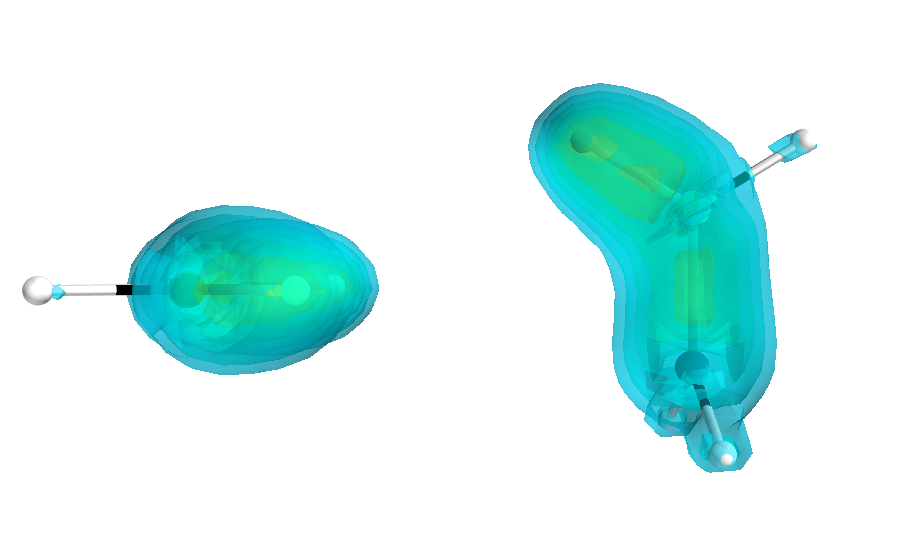
\includegraphics{Examples/C2H4_C2H4/Dyspersja_etylen.png}
\caption{Dyspersia\_etylen}
\end{figure}

    \hypertarget{wizualizacji-geminali-z-gvt-dla-wynikuxf3w-eerpa-gvb-obliczonych-za-pomocux105-dalton-oraz-gammcor}{%
\section{Wizualizacji geminali z GVT dla wyników EERPA-GVB obliczonych
za pomocą DALTON oraz
GAMMCOR}\label{wizualizacji-geminali-z-gvt-dla-wynikuxf3w-eerpa-gvb-obliczonych-za-pomocux105-dalton-oraz-gammcor}}

    W celu wizualizacji geminali początkowa część kodu wygląda analogicznie
jak w poprzednim przykładzie:

    \begin{tcolorbox}[breakable, size=fbox, boxrule=1pt, pad at break*=1mm,colback=cellbackground, colframe=cellborder]
\prompt{In}{incolor}{6}{\boxspacing}
\begin{Verbatim}[commandchars=\\\{\}]
\PY{k+kn}{import} \PY{n+nn}{visualization}\PY{n+nn}{.}\PY{n+nn}{visualization} \PY{k}{as} \PY{n+nn}{v}
\PY{k+kn}{import} \PY{n+nn}{visualization}\PY{n+nn}{.}\PY{n+nn}{dispersion\PYZus{}plot} \PY{k}{as} \PY{n+nn}{disp}
\end{Verbatim}
\end{tcolorbox}

    \begin{tcolorbox}[breakable, size=fbox, boxrule=1pt, pad at break*=1mm,colback=cellbackground, colframe=cellborder]
\prompt{In}{incolor}{7}{\boxspacing}
\begin{Verbatim}[commandchars=\\\{\}]
\PY{n}{path} \PY{o}{=} \PY{l+s+s2}{\PYZdq{}}\PY{l+s+s2}{Examples/C2H4\PYZus{}C2H4/}\PY{l+s+s2}{\PYZdq{}}
\end{Verbatim}
\end{tcolorbox}

    \begin{tcolorbox}[breakable, size=fbox, boxrule=1pt, pad at break*=1mm,colback=cellbackground, colframe=cellborder]
\prompt{In}{incolor}{10}{\boxspacing}
\begin{Verbatim}[commandchars=\\\{\}]
\PY{n}{visualization} \PY{o}{=} \PY{n}{disp}\PY{o}{.}\PY{n}{DispersionPlot}\PY{p}{(}\PY{n}{input\PYZus{}type}\PY{o}{=}\PY{l+s+s1}{\PYZsq{}}\PY{l+s+s1}{Dalton}\PY{l+s+s1}{\PYZsq{}}\PY{p}{,} \PY{n}{input\PYZus{}sub\PYZus{}type}\PY{o}{=}\PY{l+s+s1}{\PYZsq{}}\PY{l+s+s1}{tar}\PY{l+s+s1}{\PYZsq{}}\PY{p}{,}
\PY{n}{input\PYZus{}name}\PY{o}{=} \PY{n}{path} \PY{o}{+} \PY{l+s+s1}{\PYZsq{}}\PY{l+s+s1}{ethylene}\PY{l+s+s1}{\PYZsq{}}\PY{p}{)}
\PY{n}{visualization}\PY{o}{.}\PY{n}{set\PYZus{}GAMMCOR\PYZus{}filename}\PY{p}{(}\PY{n}{filename}\PY{o}{=} \PY{n}{path} \PY{o}{+} \PY{l+s+s1}{\PYZsq{}}\PY{l+s+s1}{ethylene\PYZus{}erpa.txt}\PY{l+s+s1}{\PYZsq{}}\PY{p}{)}
\end{Verbatim}
\end{tcolorbox}

    \begin{tcolorbox}[breakable, size=fbox, boxrule=1pt, pad at break*=1mm,colback=cellbackground, colframe=cellborder]
\prompt{In}{incolor}{11}{\boxspacing}
\begin{Verbatim}[commandchars=\\\{\}]
\PY{n}{visualization}\PY{o}{.}\PY{n}{get\PYZus{}dispersion\PYZus{}index}\PY{p}{(} \PY{n}{x\PYZus{}n}\PY{o}{=} \PY{l+m+mi}{100}\PY{p}{,} \PY{n}{y\PYZus{}n}\PY{o}{=} \PY{l+m+mi}{100}\PY{p}{,} \PY{n}{z\PYZus{}n}\PY{o}{=} \PY{l+m+mi}{100}\PY{p}{,} 
\PY{n}{monomer\PYZus{}A}\PY{o}{=}\PY{l+m+mi}{1}\PY{p}{,} \PY{n}{monomer\PYZus{}B}\PY{o}{=}\PY{l+m+mi}{2}\PY{p}{,} \PY{n}{gpu}\PY{o}{=}\PY{k+kc}{True}  \PY{p}{)}
\end{Verbatim}
\end{tcolorbox}

    \begin{Verbatim}[commandchars=\\\{\}]
break at line:   Sum :      -0.00094797
    \end{Verbatim}

    Następnie aby pokazać wybrany geminal należy:

    \begin{tcolorbox}[breakable, size=fbox, boxrule=1pt, pad at break*=1mm,colback=cellbackground, colframe=cellborder]
\prompt{In}{incolor}{12}{\boxspacing}
\begin{Verbatim}[commandchars=\\\{\}]
\PY{n}{figure} \PY{o}{=} \PY{n}{visualization}\PY{o}{.}\PY{n}{mlab}\PY{o}{.}\PY{n}{figure}\PY{p}{(}  \PY{l+s+s2}{\PYZdq{}}\PY{l+s+s2}{Geminal}\PY{l+s+s2}{\PYZdq{}}\PY{p}{,} 
        \PY{n}{bgcolor}\PY{o}{=} \PY{n}{visualization}\PY{o}{.}\PY{n}{visualization\PYZus{}data}\PY{o}{.}\PY{n}{background\PYZus{}colors}\PY{p}{[}\PY{l+s+s1}{\PYZsq{}}\PY{l+s+s1}{White}\PY{l+s+s1}{\PYZsq{}}\PY{p}{]}\PY{p}{,}
        \PY{n}{size}\PY{o}{=}\PY{p}{(}\PY{l+m+mi}{900}\PY{p}{,} \PY{l+m+mi}{600}\PY{p}{)} \PY{p}{)}
\PY{n}{visualization}\PY{o}{.}\PY{n}{plot\PYZus{}Geminals}\PY{p}{(} \PY{n}{geminal\PYZus{}numbers}\PY{o}{=}\PY{p}{[}\PY{l+m+mi}{11}\PY{p}{]}\PY{p}{,} \PY{n}{atom\PYZus{}names}\PY{o}{=} \PY{l+m+mi}{0}\PY{p}{,} 
\PY{n}{atom\PYZus{}scaling}\PY{o}{=} \PY{l+m+mf}{0.4}\PY{p}{,} \PY{n}{contours}\PY{o}{=}\PY{l+s+s1}{\PYZsq{}}\PY{l+s+s1}{90.0}\PY{l+s+s1}{\PYZpc{}}\PY{l+s+s1}{\PYZsq{}}\PY{p}{,} \PY{n}{plot\PYZus{}bonds}\PY{o}{=}\PY{k+kc}{True}\PY{p}{,} 
\PY{n}{bond\PYZus{}scaling} \PY{o}{=} \PY{l+m+mf}{0.4}\PY{p}{,} \PY{n}{auto\PYZus{}show}\PY{o}{=}\PY{k+kc}{False}\PY{p}{,} \PY{n}{figure}\PY{o}{=}\PY{n}{figure} \PY{p}{)}
\PY{n}{visualization}\PY{o}{.}\PY{n}{mlab}\PY{o}{.}\PY{n}{view}\PY{p}{(}\PY{n}{azimuth}\PY{o}{=}\PY{l+m+mf}{90.0}\PY{p}{,} \PY{n}{elevation}\PY{o}{=}\PY{l+m+mf}{90.0}\PY{p}{,} \PY{n}{distance}\PY{o}{=}\PY{l+m+mi}{20}\PY{p}{,} \PY{n}{focalpoint}\PY{o}{=}\PY{p}{[}\PY{o}{\PYZhy{}}\PY{l+m+mf}{3.85}\PY{p}{,} \PY{o}{\PYZhy{}}\PY{l+m+mf}{0.0}\PY{p}{,} \PY{o}{\PYZhy{}}\PY{l+m+mf}{0.0}\PY{p}{]} \PY{p}{)}
\PY{c+c1}{\PYZsh{} visualization.mlab.savefig(filename=\PYZsq{}Geminal\PYZus{}etylen.png\PYZsq{})}

\PY{n}{visualization}\PY{o}{.}\PY{n}{mlab}\PY{o}{.}\PY{n}{show}\PY{p}{(}\PY{p}{)}
\end{Verbatim}
\end{tcolorbox}

    gdzie za pomocą geminal-numbers wybieramy numer geminalu, numeracja jest
zgodna z numeracją w pliku wynikowym z programu DALTON. Użytkownik może
wyświetlić nazwy atomów (atom-names, zmienić ich rozmiar dzięki
atom-scaling, wybrać wyświetlane kontury (contours), wyświetlić wiązania
(plot-bonds) oraz zmienić ich grubość (bond-scaling). Cząsteczkę można
ustawić w przestrzeni manualnie lub też wykorzystać parametry azimuth,
elevation, distance, focalpoint. Wygenerowaną wizualizację można zapisać
w wybranym formacie, np. jako wynik.pdf. Przykład wizualizacji geminalu
pokazano poniżej.

    Oczekiwany rezultat to:

\begin{figure}
\centering
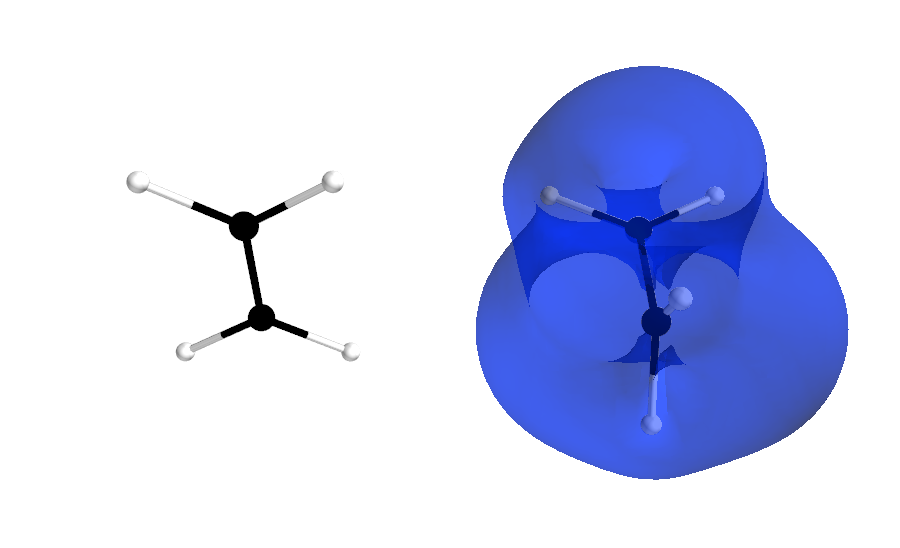
\includegraphics{Examples/C2H4_C2H4/Geminal_etylen.png}
\caption{Geminal}
\end{figure}

    \hypertarget{wizualizacji-dyspersji-z-gvt-dla-wynikuxf3w-saptcas-obliczonych-za-pomocux105-molpro-oraz-gammcor}{%
\section{Wizualizacji dyspersji z GVT dla wyników SAPT(CAS) obliczonych
za pomocą MOLPRO oraz
GAMMCOR}\label{wizualizacji-dyspersji-z-gvt-dla-wynikuxf3w-saptcas-obliczonych-za-pomocux105-molpro-oraz-gammcor}}

    \begin{tcolorbox}[breakable, size=fbox, boxrule=1pt, pad at break*=1mm,colback=cellbackground, colframe=cellborder]
\prompt{In}{incolor}{ }{\boxspacing}
\begin{Verbatim}[commandchars=\\\{\}]

\end{Verbatim}
\end{tcolorbox}

    \hypertarget{stan-podstawowy}{%
\subsection{Stan podstawowy}\label{stan-podstawowy}}

    Zaczynamy od wczytania odpowiednich modułów programu GVT:

    \begin{tcolorbox}[breakable, size=fbox, boxrule=1pt, pad at break*=1mm,colback=cellbackground, colframe=cellborder]
\prompt{In}{incolor}{13}{\boxspacing}
\begin{Verbatim}[commandchars=\\\{\}]
\PY{k+kn}{import} \PY{n+nn}{visualization}\PY{n+nn}{.}\PY{n+nn}{input\PYZus{}molpro} \PY{k}{as} \PY{n+nn}{input\PYZus{}molpro}
\PY{k+kn}{import} \PY{n+nn}{visualization}\PY{n+nn}{.}\PY{n+nn}{input\PYZus{}molpro\PYZus{}sapt} \PY{k}{as} \PY{n+nn}{input\PYZus{}sapt}
\PY{k+kn}{import} \PY{n+nn}{visualization}\PY{n+nn}{.}\PY{n+nn}{visualization} \PY{k}{as} \PY{n+nn}{V}
\PY{k+kn}{import} \PY{n+nn}{numpy} \PY{k}{as} \PY{n+nn}{np}
\PY{k+kn}{import} \PY{n+nn}{visualization}\PY{n+nn}{.}\PY{n+nn}{utils} \PY{k}{as} \PY{n+nn}{utils}
\end{Verbatim}
\end{tcolorbox}

    Wczytujemy pliki wynikowe z programów MOLPRO -- plik z rozszerzeniem
.out oraz GAMMCOR -- macierz SAPTVIS:

    \begin{tcolorbox}[breakable, size=fbox, boxrule=1pt, pad at break*=1mm,colback=cellbackground, colframe=cellborder]
\prompt{In}{incolor}{14}{\boxspacing}
\begin{Verbatim}[commandchars=\\\{\}]
\PY{n}{path\PYZus{}g} \PY{o}{=} \PY{l+s+s1}{\PYZsq{}}\PY{l+s+s1}{Examples/benzcyclo/}\PY{l+s+s1}{\PYZsq{}}
\end{Verbatim}
\end{tcolorbox}

    \begin{tcolorbox}[breakable, size=fbox, boxrule=1pt, pad at break*=1mm,colback=cellbackground, colframe=cellborder]
\prompt{In}{incolor}{15}{\boxspacing}
\begin{Verbatim}[commandchars=\\\{\}]
\PY{n}{molpro\PYZus{}output\PYZus{}file} \PY{o}{=} \PY{l+s+s1}{\PYZsq{}}\PY{l+s+s1}{benzcyclo}\PY{l+s+s1}{\PYZsq{}}
\PY{n}{sapt\PYZus{}A\PYZus{}g} \PY{o}{=} \PY{n}{V}\PY{o}{.}\PY{n}{Visualization}\PY{p}{(} \PY{n}{input\PYZus{}type}\PY{o}{=}\PY{l+s+s1}{\PYZsq{}}\PY{l+s+s1}{MolproSapt}\PY{l+s+s1}{\PYZsq{}}\PY{p}{,} \PY{n}{input\PYZus{}sub\PYZus{}type}\PY{o}{=}\PY{l+s+s1}{\PYZsq{}}\PY{l+s+s1}{output}\PY{l+s+s1}{\PYZsq{}}\PY{p}{,} \PY{n}{input\PYZus{}name}\PY{o}{=} \PY{n}{path\PYZus{}g} \PY{o}{+} \PY{n}{molpro\PYZus{}output\PYZus{}file}   \PY{p}{)}
\PY{n}{sapt\PYZus{}B\PYZus{}g} \PY{o}{=} \PY{n}{V}\PY{o}{.}\PY{n}{Visualization}\PY{p}{(} \PY{n}{input\PYZus{}type}\PY{o}{=}\PY{l+s+s1}{\PYZsq{}}\PY{l+s+s1}{MolproSapt}\PY{l+s+s1}{\PYZsq{}}\PY{p}{,} \PY{n}{input\PYZus{}sub\PYZus{}type}\PY{o}{=}\PY{l+s+s1}{\PYZsq{}}\PY{l+s+s1}{output}\PY{l+s+s1}{\PYZsq{}}\PY{p}{,} \PY{n}{input\PYZus{}name}\PY{o}{=} \PY{n}{path\PYZus{}g} \PY{o}{+} \PY{n}{molpro\PYZus{}output\PYZus{}file}   \PY{p}{)}
\PY{n}{sapt\PYZus{}B\PYZus{}g}\PY{o}{.}\PY{n}{data\PYZus{}input}\PY{o}{.}\PY{n}{monomer} \PY{o}{=} \PY{l+m+mi}{1} 
\end{Verbatim}
\end{tcolorbox}

    Program GVT powinien w kolejnym kroku przeczytać geometrie dla obu
monomerów, ładunki oraz dane opisujące orbitale:

    \begin{tcolorbox}[breakable, size=fbox, boxrule=1pt, pad at break*=1mm,colback=cellbackground, colframe=cellborder]
\prompt{In}{incolor}{16}{\boxspacing}
\begin{Verbatim}[commandchars=\\\{\}]
\PY{n}{sapt\PYZus{}A\PYZus{}g}\PY{o}{.}\PY{n}{get\PYZus{}geometry}\PY{p}{(}\PY{p}{)}
\PY{n}{sapt\PYZus{}B\PYZus{}g}\PY{o}{.}\PY{n}{get\PYZus{}geometry}\PY{p}{(}\PY{p}{)}
\PY{n}{sapt\PYZus{}A\PYZus{}g}\PY{o}{.}\PY{n}{molecular\PYZus{}system}\PY{o}{.}\PY{n}{atoms\PYZus{}Charge}
\PY{n}{sapt\PYZus{}B\PYZus{}g}\PY{o}{.}\PY{n}{molecular\PYZus{}system}\PY{o}{.}\PY{n}{atoms\PYZus{}Charge}
\PY{n}{sapt\PYZus{}A\PYZus{}g}\PY{o}{.}\PY{n}{get\PYZus{}orbital\PYZus{}data}\PY{p}{(} \PY{p}{)}
\end{Verbatim}
\end{tcolorbox}

    Następnie należy ustawić dokładność grida dla prezentacji wyników. Im
większe wartości dla x-n, y-n i z-n wybierzemy tym grid będzie
dokładniejszy, jednak będzie wymagał znacznie dłuższego wczytywania
danych. Proponujemy zacząć od wartości 10 dla wszystkich trzech
parametrów, a następnie zwiększyć dokładność wyświetlania.

    \begin{tcolorbox}[breakable, size=fbox, boxrule=1pt, pad at break*=1mm,colback=cellbackground, colframe=cellborder]
\prompt{In}{incolor}{17}{\boxspacing}
\begin{Verbatim}[commandchars=\\\{\}]
\PY{n}{sapt\PYZus{}A\PYZus{}g}\PY{o}{.}\PY{n}{orbital\PYZus{}generator}\PY{o}{.}\PY{n}{grid}\PY{o}{.}\PY{n}{R\PYZus{}max\PYZus{}multip} \PY{o}{=} \PY{l+m+mf}{1.5}
\PY{n}{sapt\PYZus{}A\PYZus{}g}\PY{o}{.}\PY{n}{orbital\PYZus{}generator}\PY{o}{.}\PY{n}{grid}\PY{o}{.}\PY{n}{x\PYZus{}n} \PY{o}{=} \PY{l+m+mi}{50}
\PY{n}{sapt\PYZus{}A\PYZus{}g}\PY{o}{.}\PY{n}{orbital\PYZus{}generator}\PY{o}{.}\PY{n}{grid}\PY{o}{.}\PY{n}{y\PYZus{}n} \PY{o}{=} \PY{l+m+mi}{50}
\PY{n}{sapt\PYZus{}A\PYZus{}g}\PY{o}{.}\PY{n}{orbital\PYZus{}generator}\PY{o}{.}\PY{n}{grid}\PY{o}{.}\PY{n}{z\PYZus{}n} \PY{o}{=} \PY{l+m+mi}{50}
\PY{n}{sapt\PYZus{}A\PYZus{}g}\PY{o}{.}\PY{n}{orbital\PYZus{}generator}\PY{o}{.}\PY{n}{init\PYZus{}grid}\PY{p}{(} \PY{p}{)}
\PY{n}{sapt\PYZus{}A\PYZus{}g}\PY{o}{.}\PY{n}{orbital\PYZus{}generator}\PY{o}{.}\PY{n}{init\PYZus{}AOs}\PY{p}{(}\PY{p}{)}
\PY{n}{sapt\PYZus{}A\PYZus{}g}\PY{o}{.}\PY{n}{orbital\PYZus{}generator}\PY{o}{.}\PY{n}{spherical}  \PY{o}{=} \PY{l+m+mi}{1} 
\PY{n}{sapt\PYZus{}B\PYZus{}g}\PY{o}{.}\PY{n}{get\PYZus{}orbital\PYZus{}data}\PY{p}{(} \PY{p}{)}
\PY{n}{sapt\PYZus{}B\PYZus{}g}\PY{o}{.}\PY{n}{orbital\PYZus{}generator}\PY{o}{.}\PY{n}{grid}\PY{o}{.}\PY{n}{R\PYZus{}max\PYZus{}multip} \PY{o}{=} \PY{l+m+mf}{1.5}
\PY{n}{sapt\PYZus{}B\PYZus{}g}\PY{o}{.}\PY{n}{orbital\PYZus{}generator}\PY{o}{.}\PY{n}{grid}\PY{o}{.}\PY{n}{x\PYZus{}n} \PY{o}{=} \PY{l+m+mi}{50}
\PY{n}{sapt\PYZus{}B\PYZus{}g}\PY{o}{.}\PY{n}{orbital\PYZus{}generator}\PY{o}{.}\PY{n}{grid}\PY{o}{.}\PY{n}{y\PYZus{}n} \PY{o}{=} \PY{l+m+mi}{50}
\PY{n}{sapt\PYZus{}B\PYZus{}g}\PY{o}{.}\PY{n}{orbital\PYZus{}generator}\PY{o}{.}\PY{n}{grid}\PY{o}{.}\PY{n}{z\PYZus{}n} \PY{o}{=} \PY{l+m+mi}{50}
\PY{n}{sapt\PYZus{}B\PYZus{}g}\PY{o}{.}\PY{n}{orbital\PYZus{}generator}\PY{o}{.}\PY{n}{init\PYZus{}grid}\PY{p}{(} \PY{p}{)}
\PY{n}{sapt\PYZus{}B\PYZus{}g}\PY{o}{.}\PY{n}{orbital\PYZus{}generator}\PY{o}{.}\PY{n}{init\PYZus{}AOs}\PY{p}{(}\PY{p}{)}
\PY{n}{sapt\PYZus{}B\PYZus{}g}\PY{o}{.}\PY{n}{orbital\PYZus{}generator}\PY{o}{.}\PY{n}{spherical}  \PY{o}{=} \PY{k+kc}{True} 
\end{Verbatim}
\end{tcolorbox}

    Dalsza część kodu przetwarza współczynniki rozwinięć, generuje dane dla
orbitali atomowych AO oraz orbitali molekularnych MO:

    \begin{tcolorbox}[breakable, size=fbox, boxrule=1pt, pad at break*=1mm,colback=cellbackground, colframe=cellborder]
\prompt{In}{incolor}{18}{\boxspacing}
\begin{Verbatim}[commandchars=\\\{\}]
\PY{n}{ANBasis\PYZus{}g}\PY{p}{,} \PY{n}{BNBasis\PYZus{}g}\PY{p}{,} \PY{n}{NOccupA\PYZus{}g}\PY{p}{,} \PY{n}{NOccupB\PYZus{}g}\PY{p}{,} \PY{n}{A\PYZus{}Occ\PYZus{}g}\PY{p}{,} \PY{n}{B\PYZus{}Occ\PYZus{}g}\PY{p}{,} \PY{n}{ACMO\PYZus{}g}\PY{p}{,} \PY{n}{BCMO\PYZus{}g}\PY{p}{,} \PY{n}{Qmat\PYZus{}g} \PY{o}{=} \PY{n}{utils}\PY{o}{.}\PY{n}{read\PYZus{}SAPTVIS}\PY{p}{(} \PY{n}{path\PYZus{}g} \PY{o}{+} \PY{l+s+s1}{\PYZsq{}}\PY{l+s+s1}{SAPTVIS}\PY{l+s+s1}{\PYZsq{}} \PY{p}{)}
\PY{n}{sapt\PYZus{}A\PYZus{}g}\PY{o}{.}\PY{n}{molecular\PYZus{}system}\PY{o}{.}\PY{n}{Coeff}\PY{p}{[}\PY{p}{:}\PY{p}{,}\PY{p}{:}\PY{p}{]} \PY{o}{=} \PY{n}{ACMO\PYZus{}g}
\PY{n}{sapt\PYZus{}B\PYZus{}g}\PY{o}{.}\PY{n}{molecular\PYZus{}system}\PY{o}{.}\PY{n}{Coeff}\PY{p}{[}\PY{p}{:}\PY{p}{,}\PY{p}{:}\PY{p}{]} \PY{o}{=} \PY{n}{BCMO\PYZus{}g}
\PY{n}{sapt\PYZus{}A\PYZus{}g}\PY{o}{.}\PY{n}{generate\PYZus{}AO\PYZus{}orbitals\PYZus{}gpu}\PY{p}{(}\PY{p}{)}
\PY{n}{sapt\PYZus{}A\PYZus{}g}\PY{o}{.}\PY{n}{generate\PYZus{}MO\PYZus{}orbitals\PYZus{}gpu}\PY{p}{(}\PY{p}{)}
\PY{n}{sapt\PYZus{}B\PYZus{}g}\PY{o}{.}\PY{n}{generate\PYZus{}AO\PYZus{}orbitals\PYZus{}gpu}\PY{p}{(}\PY{p}{)}
\PY{n}{sapt\PYZus{}B\PYZus{}g}\PY{o}{.}\PY{n}{generate\PYZus{}MO\PYZus{}orbitals\PYZus{}gpu}\PY{p}{(}\PY{p}{)}
\end{Verbatim}
\end{tcolorbox}

    Następnie obliczamy macierz Q na podstawie której wyświetlać będziemy
dyspersję:

    \begin{tcolorbox}[breakable, size=fbox, boxrule=1pt, pad at break*=1mm,colback=cellbackground, colframe=cellborder]
\prompt{In}{incolor}{19}{\boxspacing}
\begin{Verbatim}[commandchars=\\\{\}]
\PY{n}{sapt\PYZus{}dispersion\PYZus{}A\PYZus{}g} \PY{o}{=}  \PY{n}{np}\PY{o}{.}\PY{n}{zeros\PYZus{}like}\PY{p}{(} \PY{n}{sapt\PYZus{}A\PYZus{}g}\PY{o}{.}\PY{n}{molecular\PYZus{}system}\PY{o}{.}\PY{n}{AOs}\PY{p}{[}\PY{l+m+mi}{0}\PY{p}{]} \PY{p}{)}
\PY{n}{sapt\PYZus{}dispersion\PYZus{}B\PYZus{}g} \PY{o}{=}  \PY{n}{np}\PY{o}{.}\PY{n}{zeros\PYZus{}like}\PY{p}{(} \PY{n}{sapt\PYZus{}B\PYZus{}g}\PY{o}{.}\PY{n}{molecular\PYZus{}system}\PY{o}{.}\PY{n}{AOs}\PY{p}{[}\PY{l+m+mi}{0}\PY{p}{]} \PY{p}{)}
\PY{n}{Qmat\PYZus{}tmp\PYZus{}g} \PY{o}{=} \PY{n}{np}\PY{o}{.}\PY{n}{reshape}\PY{p}{(}\PY{n}{Qmat\PYZus{}g}\PY{p}{,} \PY{p}{[}\PY{n}{NOccupB\PYZus{}g}\PY{p}{,}\PY{n}{NOccupA\PYZus{}g}\PY{p}{]} \PY{p}{)}\PY{o}{.}\PY{n}{transpose}\PY{p}{(}\PY{p}{)}
\PY{k}{for} \PY{n}{i} \PY{o+ow}{in} \PY{n+nb}{range}\PY{p}{(}\PY{n}{NOccupA\PYZus{}g}\PY{p}{)}\PY{p}{:}
    \PY{k}{for} \PY{n}{j} \PY{o+ow}{in} \PY{n+nb}{range}\PY{p}{(}\PY{n}{NOccupB\PYZus{}g}\PY{p}{)}\PY{p}{:}   
        \PY{n}{sapt\PYZus{}dispersion\PYZus{}A\PYZus{}g} \PY{o}{+}\PY{o}{=} \PY{n}{Qmat\PYZus{}tmp\PYZus{}g}\PY{p}{[}\PY{n}{i}\PY{p}{,}\PY{n}{j}\PY{p}{]} \PY{o}{*} \PY{n}{A\PYZus{}Occ\PYZus{}g}\PY{p}{[}\PY{n}{i}\PY{p}{]} \PY{o}{*} \PY{n}{sapt\PYZus{}A\PYZus{}g}\PY{o}{.}\PY{n}{molecular\PYZus{}system}\PY{o}{.}\PY{n}{MOs}\PY{p}{[}\PY{n}{i}\PY{p}{]}\PY{o}{*}\PY{o}{*}\PY{l+m+mi}{2} 
        \PY{n}{sapt\PYZus{}dispersion\PYZus{}B\PYZus{}g} \PY{o}{+}\PY{o}{=} \PY{n}{Qmat\PYZus{}tmp\PYZus{}g}\PY{p}{[}\PY{n}{i}\PY{p}{,}\PY{n}{j}\PY{p}{]} \PY{o}{*} \PY{n}{B\PYZus{}Occ\PYZus{}g}\PY{p}{[}\PY{n}{j}\PY{p}{]} \PY{o}{*} \PY{n}{sapt\PYZus{}B\PYZus{}g}\PY{o}{.}\PY{n}{molecular\PYZus{}system}\PY{o}{.}\PY{n}{MOs}\PY{p}{[}\PY{n}{j}\PY{p}{]}\PY{o}{*}\PY{o}{*}\PY{l+m+mi}{2} 
\PY{n}{sapt\PYZus{}dispersion\PYZus{}AB\PYZus{}g} \PY{o}{=} \PY{o}{\PYZhy{}}\PY{l+m+mf}{0.5} \PY{o}{*} \PY{p}{(} \PY{n}{sapt\PYZus{}dispersion\PYZus{}A\PYZus{}g} \PY{o}{+} \PY{n}{sapt\PYZus{}dispersion\PYZus{}B\PYZus{}g} \PY{p}{)}  
\end{Verbatim}
\end{tcolorbox}

    Do tej pory zmiany w kodzie wymagała jedynie nazwa folderu z plikami
wynikowymi oraz nazwa plików wynikowych, a także gęstość grida. W
ostatniej części kodu znów możemy manipulować parametrami takimi jak
wyświetlanie wiązań oraz ustawienie ich grubości, ustawienie wielkości
atomów, rodzaju i ilości konturów:

    \begin{tcolorbox}[breakable, size=fbox, boxrule=1pt, pad at break*=1mm,colback=cellbackground, colframe=cellborder]
\prompt{In}{incolor}{20}{\boxspacing}
\begin{Verbatim}[commandchars=\\\{\}]
\PY{n}{X}\PY{p}{,} \PY{n}{Y}\PY{p}{,} \PY{n}{Z} \PY{o}{=} \PY{n}{sapt\PYZus{}A\PYZus{}g}\PY{o}{.}\PY{n}{orbital\PYZus{}generator}\PY{o}{.}\PY{n}{grid}\PY{o}{.}\PY{n}{return\PYZus{}grid\PYZus{}arrays}\PY{p}{(}\PY{p}{)}
\PY{n}{figure} \PY{o}{=} \PY{n}{visualization}\PY{o}{.}\PY{n}{mlab}\PY{o}{.}\PY{n}{figure}\PY{p}{(}  \PY{l+s+s2}{\PYZdq{}}\PY{l+s+s2}{sapt\PYZus{}dispersion\PYZus{}AB\PYZus{}g}\PY{l+s+s2}{\PYZdq{}}\PY{p}{,} 
        \PY{n}{bgcolor}\PY{o}{=} \PY{n}{visualization}\PY{o}{.}\PY{n}{visualization\PYZus{}data}\PY{o}{.}\PY{n}{background\PYZus{}colors}\PY{p}{[}\PY{l+s+s1}{\PYZsq{}}\PY{l+s+s1}{White}\PY{l+s+s1}{\PYZsq{}}\PY{p}{]}\PY{p}{,}
        \PY{n}{size}\PY{o}{=}\PY{p}{(}\PY{l+m+mi}{900}\PY{p}{,} \PY{l+m+mi}{600}\PY{p}{)} \PY{p}{)}
\PY{n}{plot\PYZus{}figure} \PY{o}{=} \PY{n}{sapt\PYZus{}A\PYZus{}g}\PY{o}{.}\PY{n}{plot\PYZus{}orbitals\PYZus{}MO}\PY{p}{(}\PY{n}{orbital\PYZus{}numbers}\PY{o}{=}\PY{p}{[}\PY{p}{]}\PY{p}{,}\PY{n}{auto\PYZus{}show}\PY{o}{=}\PY{k+kc}{False}\PY{p}{,} 
    \PY{n}{plot\PYZus{}bonds}\PY{o}{=}\PY{k+kc}{True}\PY{p}{,} \PY{n}{atom\PYZus{}names}\PY{o}{=}\PY{k+kc}{False}\PY{p}{,} \PY{n}{atom\PYZus{}scaling}\PY{o}{=}\PY{l+m+mf}{0.5}\PY{p}{,} \PY{n}{figure}\PY{o}{=}\PY{n}{figure} \PY{p}{)}
\PY{n}{sapt\PYZus{}A\PYZus{}g}\PY{o}{.}\PY{n}{mlab}\PY{o}{.}\PY{n}{contour3d}\PY{p}{(} \PY{n}{X}\PY{p}{,} \PY{n}{Y}\PY{p}{,} \PY{n}{Z}\PY{p}{,} \PY{n}{sapt\PYZus{}dispersion\PYZus{}AB\PYZus{}g}\PY{p}{,}  
    \PY{n}{contours}\PY{o}{=} \PY{n}{sapt\PYZus{}A\PYZus{}g}\PY{o}{.}\PY{n}{contour\PYZus{}process}\PY{p}{(}\PY{p}{[}\PY{l+s+s1}{\PYZsq{}}\PY{l+s+s1}{50}\PY{l+s+s1}{\PYZpc{}}\PY{l+s+s1}{\PYZsq{}}\PY{p}{,}\PY{l+s+s1}{\PYZsq{}}\PY{l+s+s1}{40}\PY{l+s+s1}{\PYZpc{}}\PY{l+s+s1}{\PYZsq{}}\PY{p}{,}\PY{l+s+s1}{\PYZsq{}}\PY{l+s+s1}{30}\PY{l+s+s1}{\PYZpc{}}\PY{l+s+s1}{\PYZsq{}}\PY{p}{,}\PY{l+s+s1}{\PYZsq{}}\PY{l+s+s1}{20}\PY{l+s+s1}{\PYZpc{}}\PY{l+s+s1}{\PYZsq{}}\PY{p}{,}\PY{l+s+s1}{\PYZsq{}}\PY{l+s+s1}{10}\PY{l+s+s1}{\PYZpc{}}\PY{l+s+s1}{\PYZsq{}}\PY{p}{,}\PY{l+s+s1}{\PYZsq{}}\PY{l+s+s1}{1}\PY{l+s+s1}{\PYZpc{}}\PY{l+s+s1}{\PYZsq{}}\PY{p}{]}\PY{p}{,} 
    \PY{n}{sapt\PYZus{}dispersion\PYZus{}AB\PYZus{}g}\PY{p}{)} \PY{p}{,} \PY{n}{opacity}\PY{o}{=}\PY{l+m+mf}{0.5}\PY{p}{)}
\PY{n}{sapt\PYZus{}A\PYZus{}g}\PY{o}{.}\PY{n}{mlab}\PY{o}{.}\PY{n}{view}\PY{p}{(} \PY{n}{distance}\PY{o}{=}\PY{l+m+mi}{26} \PY{p}{)}
\PY{c+c1}{\PYZsh{} sapt\PYZus{}A\PYZus{}g.mlab.savefig(filename= \PYZsq{}sapt\PYZus{}dispersion\PYZus{}AB\PYZus{}g.png\PYZsq{})}

\PY{n}{sapt\PYZus{}A\PYZus{}g}\PY{o}{.}\PY{n}{mlab}\PY{o}{.}\PY{n}{show}\PY{p}{(}\PY{p}{)}
\end{Verbatim}
\end{tcolorbox}

    Przykład wizualizacji dyspersji dla stanu podstawowego układu
benzen-cyklopentan pokazano poniżej:

\begin{figure}
\centering
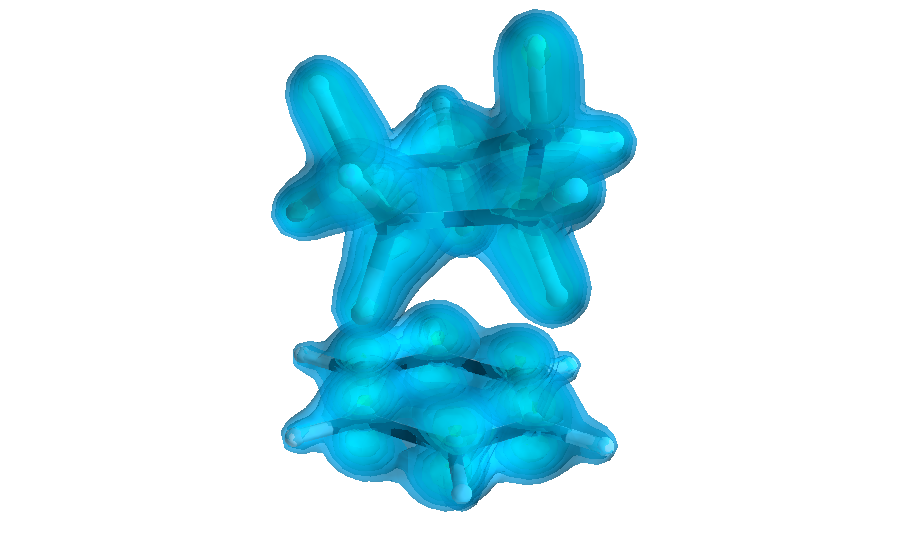
\includegraphics{Examples/benzcyclo/sapt_dispersion_AB_g.png}
\caption{sapt\_dispersion\_AB\_g}
\end{figure}

    \hypertarget{stan-wzbudzony}{%
\subsection{Stan wzbudzony}\label{stan-wzbudzony}}

    Postępujemy analogicznie jak dla stanu podstawowego.

    \begin{tcolorbox}[breakable, size=fbox, boxrule=1pt, pad at break*=1mm,colback=cellbackground, colframe=cellborder]
\prompt{In}{incolor}{21}{\boxspacing}
\begin{Verbatim}[commandchars=\\\{\}]
\PY{n}{path\PYZus{}e} \PY{o}{=} \PY{l+s+s1}{\PYZsq{}}\PY{l+s+s1}{Examples/benzcyclo\PYZus{}excite/}\PY{l+s+s1}{\PYZsq{}}
\end{Verbatim}
\end{tcolorbox}

    \begin{tcolorbox}[breakable, size=fbox, boxrule=1pt, pad at break*=1mm,colback=cellbackground, colframe=cellborder]
\prompt{In}{incolor}{22}{\boxspacing}
\begin{Verbatim}[commandchars=\\\{\}]
\PY{n}{molpro\PYZus{}output\PYZus{}file} \PY{o}{=} \PY{l+s+s1}{\PYZsq{}}\PY{l+s+s1}{benzcyclo}\PY{l+s+s1}{\PYZsq{}}
\PY{n}{sapt\PYZus{}A\PYZus{}e} \PY{o}{=} \PY{n}{V}\PY{o}{.}\PY{n}{Visualization}\PY{p}{(} \PY{n}{input\PYZus{}type}\PY{o}{=}\PY{l+s+s1}{\PYZsq{}}\PY{l+s+s1}{MolproSapt}\PY{l+s+s1}{\PYZsq{}}\PY{p}{,} \PY{n}{input\PYZus{}sub\PYZus{}type}\PY{o}{=}\PY{l+s+s1}{\PYZsq{}}\PY{l+s+s1}{output}\PY{l+s+s1}{\PYZsq{}}\PY{p}{,}  
\PY{n}{input\PYZus{}name}\PY{o}{=} \PY{n}{path\PYZus{}e} \PY{o}{+} \PY{n}{molpro\PYZus{}output\PYZus{}file}   \PY{p}{)}
\PY{n}{sapt\PYZus{}B\PYZus{}e} \PY{o}{=} \PY{n}{V}\PY{o}{.}\PY{n}{Visualization}\PY{p}{(} \PY{n}{input\PYZus{}type}\PY{o}{=}\PY{l+s+s1}{\PYZsq{}}\PY{l+s+s1}{MolproSapt}\PY{l+s+s1}{\PYZsq{}}\PY{p}{,} \PY{n}{input\PYZus{}sub\PYZus{}type}\PY{o}{=}\PY{l+s+s1}{\PYZsq{}}\PY{l+s+s1}{output}\PY{l+s+s1}{\PYZsq{}}\PY{p}{,}  
\PY{n}{input\PYZus{}name}\PY{o}{=} \PY{n}{path\PYZus{}e} \PY{o}{+} \PY{n}{molpro\PYZus{}output\PYZus{}file}   \PY{p}{)}
\PY{n}{sapt\PYZus{}B\PYZus{}e}\PY{o}{.}\PY{n}{data\PYZus{}input}\PY{o}{.}\PY{n}{monomer} \PY{o}{=} \PY{l+m+mi}{1} 
\end{Verbatim}
\end{tcolorbox}

    \begin{tcolorbox}[breakable, size=fbox, boxrule=1pt, pad at break*=1mm,colback=cellbackground, colframe=cellborder]
\prompt{In}{incolor}{23}{\boxspacing}
\begin{Verbatim}[commandchars=\\\{\}]
\PY{n}{sapt\PYZus{}A\PYZus{}e}\PY{o}{.}\PY{n}{get\PYZus{}geometry}\PY{p}{(}\PY{p}{)}
\PY{n}{sapt\PYZus{}B\PYZus{}e}\PY{o}{.}\PY{n}{get\PYZus{}geometry}\PY{p}{(}\PY{p}{)}
\PY{n}{sapt\PYZus{}A\PYZus{}e}\PY{o}{.}\PY{n}{molecular\PYZus{}system}\PY{o}{.}\PY{n}{atoms\PYZus{}Charge}
\PY{n}{sapt\PYZus{}B\PYZus{}e}\PY{o}{.}\PY{n}{molecular\PYZus{}system}\PY{o}{.}\PY{n}{atoms\PYZus{}Charge}
\PY{n}{sapt\PYZus{}A\PYZus{}e}\PY{o}{.}\PY{n}{get\PYZus{}orbital\PYZus{}data}\PY{p}{(} \PY{p}{)}
\PY{n}{sapt\PYZus{}A\PYZus{}e}\PY{o}{.}\PY{n}{orbital\PYZus{}generator}\PY{o}{.}\PY{n}{grid}\PY{o}{.}\PY{n}{R\PYZus{}max\PYZus{}multip} \PY{o}{=} \PY{l+m+mf}{1.5}
\PY{n}{sapt\PYZus{}A\PYZus{}e}\PY{o}{.}\PY{n}{orbital\PYZus{}generator}\PY{o}{.}\PY{n}{grid}\PY{o}{.}\PY{n}{x\PYZus{}n} \PY{o}{=} \PY{l+m+mi}{50}
\PY{n}{sapt\PYZus{}A\PYZus{}e}\PY{o}{.}\PY{n}{orbital\PYZus{}generator}\PY{o}{.}\PY{n}{grid}\PY{o}{.}\PY{n}{y\PYZus{}n} \PY{o}{=} \PY{l+m+mi}{50}
\PY{n}{sapt\PYZus{}A\PYZus{}e}\PY{o}{.}\PY{n}{orbital\PYZus{}generator}\PY{o}{.}\PY{n}{grid}\PY{o}{.}\PY{n}{z\PYZus{}n} \PY{o}{=} \PY{l+m+mi}{50}
\PY{n}{sapt\PYZus{}A\PYZus{}e}\PY{o}{.}\PY{n}{orbital\PYZus{}generator}\PY{o}{.}\PY{n}{init\PYZus{}grid}\PY{p}{(} \PY{p}{)}
\PY{n}{sapt\PYZus{}A\PYZus{}e}\PY{o}{.}\PY{n}{orbital\PYZus{}generator}\PY{o}{.}\PY{n}{init\PYZus{}AOs}\PY{p}{(}\PY{p}{)}
\PY{n}{sapt\PYZus{}A\PYZus{}e}\PY{o}{.}\PY{n}{orbital\PYZus{}generator}\PY{o}{.}\PY{n}{spherical}  \PY{o}{=} \PY{l+m+mi}{1} 
\PY{n}{sapt\PYZus{}B\PYZus{}e}\PY{o}{.}\PY{n}{get\PYZus{}orbital\PYZus{}data}\PY{p}{(} \PY{p}{)}
\PY{n}{sapt\PYZus{}B\PYZus{}e}\PY{o}{.}\PY{n}{orbital\PYZus{}generator}\PY{o}{.}\PY{n}{grid}\PY{o}{.}\PY{n}{R\PYZus{}max\PYZus{}multip} \PY{o}{=} \PY{l+m+mf}{1.5}
\PY{n}{sapt\PYZus{}B\PYZus{}e}\PY{o}{.}\PY{n}{orbital\PYZus{}generator}\PY{o}{.}\PY{n}{grid}\PY{o}{.}\PY{n}{x\PYZus{}n} \PY{o}{=} \PY{l+m+mi}{50}
\PY{n}{sapt\PYZus{}B\PYZus{}e}\PY{o}{.}\PY{n}{orbital\PYZus{}generator}\PY{o}{.}\PY{n}{grid}\PY{o}{.}\PY{n}{y\PYZus{}n} \PY{o}{=} \PY{l+m+mi}{50}
\PY{n}{sapt\PYZus{}B\PYZus{}e}\PY{o}{.}\PY{n}{orbital\PYZus{}generator}\PY{o}{.}\PY{n}{grid}\PY{o}{.}\PY{n}{z\PYZus{}n} \PY{o}{=} \PY{l+m+mi}{50}
\PY{n}{sapt\PYZus{}B\PYZus{}e}\PY{o}{.}\PY{n}{orbital\PYZus{}generator}\PY{o}{.}\PY{n}{init\PYZus{}grid}\PY{p}{(} \PY{p}{)}
\PY{n}{sapt\PYZus{}B\PYZus{}e}\PY{o}{.}\PY{n}{orbital\PYZus{}generator}\PY{o}{.}\PY{n}{init\PYZus{}AOs}\PY{p}{(}\PY{p}{)}
\PY{n}{sapt\PYZus{}B\PYZus{}e}\PY{o}{.}\PY{n}{orbital\PYZus{}generator}\PY{o}{.}\PY{n}{spherical}  \PY{o}{=} \PY{l+m+mi}{1} 
\end{Verbatim}
\end{tcolorbox}

    \begin{tcolorbox}[breakable, size=fbox, boxrule=1pt, pad at break*=1mm,colback=cellbackground, colframe=cellborder]
\prompt{In}{incolor}{24}{\boxspacing}
\begin{Verbatim}[commandchars=\\\{\}]
\PY{n}{ANBasis\PYZus{}e}\PY{p}{,} \PY{n}{BNBasis\PYZus{}e}\PY{p}{,} \PY{n}{NOccupA\PYZus{}e}\PY{p}{,} \PY{n}{NOccupB\PYZus{}e}\PY{p}{,} \PY{n}{A\PYZus{}Occ\PYZus{}e}\PY{p}{,} \PY{n}{B\PYZus{}Occ\PYZus{}e}\PY{p}{,} \PY{n}{ACMO\PYZus{}e}\PY{p}{,} \PY{n}{BCMO\PYZus{}e}\PY{p}{,} \PY{n}{Qmat\PYZus{}e} \PY{o}{=} \PY{n}{utils}\PY{o}{.}\PY{n}{read\PYZus{}SAPTVIS}\PY{p}{(} \PY{n}{path\PYZus{}e} \PY{o}{+} \PY{l+s+s1}{\PYZsq{}}\PY{l+s+s1}{SAPTVIS}\PY{l+s+s1}{\PYZsq{}} \PY{p}{)}
\PY{n}{sapt\PYZus{}A\PYZus{}e}\PY{o}{.}\PY{n}{molecular\PYZus{}system}\PY{o}{.}\PY{n}{Coeff}\PY{p}{[}\PY{p}{:}\PY{p}{,}\PY{p}{:}\PY{p}{]} \PY{o}{=} \PY{n}{ACMO\PYZus{}e}
\PY{n}{sapt\PYZus{}B\PYZus{}e}\PY{o}{.}\PY{n}{molecular\PYZus{}system}\PY{o}{.}\PY{n}{Coeff}\PY{p}{[}\PY{p}{:}\PY{p}{,}\PY{p}{:}\PY{p}{]} \PY{o}{=} \PY{n}{BCMO\PYZus{}e}
\PY{n}{sapt\PYZus{}A\PYZus{}e}\PY{o}{.}\PY{n}{generate\PYZus{}AO\PYZus{}orbitals\PYZus{}gpu}\PY{p}{(}\PY{p}{)}
\PY{n}{sapt\PYZus{}A\PYZus{}e}\PY{o}{.}\PY{n}{generate\PYZus{}MO\PYZus{}orbitals\PYZus{}gpu}\PY{p}{(}\PY{p}{)}
\PY{n}{sapt\PYZus{}B\PYZus{}e}\PY{o}{.}\PY{n}{generate\PYZus{}AO\PYZus{}orbitals\PYZus{}gpu}\PY{p}{(}\PY{p}{)}
\PY{n}{sapt\PYZus{}B\PYZus{}e}\PY{o}{.}\PY{n}{generate\PYZus{}MO\PYZus{}orbitals\PYZus{}gpu}\PY{p}{(}\PY{p}{)}
\end{Verbatim}
\end{tcolorbox}

    \begin{tcolorbox}[breakable, size=fbox, boxrule=1pt, pad at break*=1mm,colback=cellbackground, colframe=cellborder]
\prompt{In}{incolor}{25}{\boxspacing}
\begin{Verbatim}[commandchars=\\\{\}]
\PY{n}{sapt\PYZus{}dispersion\PYZus{}A\PYZus{}e} \PY{o}{=}  \PY{n}{np}\PY{o}{.}\PY{n}{zeros\PYZus{}like}\PY{p}{(} \PY{n}{sapt\PYZus{}A\PYZus{}e}\PY{o}{.}\PY{n}{molecular\PYZus{}system}\PY{o}{.}\PY{n}{AOs}\PY{p}{[}\PY{l+m+mi}{0}\PY{p}{]} \PY{p}{)}
\PY{n}{sapt\PYZus{}dispersion\PYZus{}B\PYZus{}e} \PY{o}{=}  \PY{n}{np}\PY{o}{.}\PY{n}{zeros\PYZus{}like}\PY{p}{(} \PY{n}{sapt\PYZus{}B\PYZus{}e}\PY{o}{.}\PY{n}{molecular\PYZus{}system}\PY{o}{.}\PY{n}{AOs}\PY{p}{[}\PY{l+m+mi}{0}\PY{p}{]} \PY{p}{)}
\PY{n}{Qmat\PYZus{}tmp\PYZus{}e} \PY{o}{=} \PY{n}{np}\PY{o}{.}\PY{n}{reshape}\PY{p}{(}\PY{n}{Qmat\PYZus{}e}\PY{p}{,} \PY{p}{[}\PY{n}{NOccupB\PYZus{}e}\PY{p}{,}\PY{n}{NOccupA\PYZus{}e}\PY{p}{]} \PY{p}{)}\PY{o}{.}\PY{n}{transpose}\PY{p}{(}\PY{p}{)}
\PY{k}{for} \PY{n}{i} \PY{o+ow}{in} \PY{n+nb}{range}\PY{p}{(}\PY{n}{NOccupA\PYZus{}e}\PY{p}{)}\PY{p}{:}
\PY{c+c1}{\PYZsh{}     print(i)}
    \PY{k}{for} \PY{n}{j} \PY{o+ow}{in} \PY{n+nb}{range}\PY{p}{(}\PY{n}{NOccupB\PYZus{}e}\PY{p}{)}\PY{p}{:}      
        \PY{n}{sapt\PYZus{}dispersion\PYZus{}A\PYZus{}e} \PY{o}{+}\PY{o}{=} \PY{n}{Qmat\PYZus{}tmp\PYZus{}e}\PY{p}{[}\PY{n}{i}\PY{p}{,}\PY{n}{j}\PY{p}{]} \PY{o}{*} \PY{n}{A\PYZus{}Occ\PYZus{}e}\PY{p}{[}\PY{n}{i}\PY{p}{]} \PY{o}{*} \PY{n}{sapt\PYZus{}A\PYZus{}e}\PY{o}{.}\PY{n}{molecular\PYZus{}system}\PY{o}{.}\PY{n}{MOs}\PY{p}{[}\PY{n}{i}\PY{p}{]}\PY{o}{*}\PY{o}{*}\PY{l+m+mi}{2} 
        \PY{n}{sapt\PYZus{}dispersion\PYZus{}B\PYZus{}e} \PY{o}{+}\PY{o}{=} \PY{n}{Qmat\PYZus{}tmp\PYZus{}e}\PY{p}{[}\PY{n}{i}\PY{p}{,}\PY{n}{j}\PY{p}{]} \PY{o}{*} \PY{n}{B\PYZus{}Occ\PYZus{}e}\PY{p}{[}\PY{n}{j}\PY{p}{]} \PY{o}{*} \PY{n}{sapt\PYZus{}B\PYZus{}e}\PY{o}{.}\PY{n}{molecular\PYZus{}system}\PY{o}{.}\PY{n}{MOs}\PY{p}{[}\PY{n}{j}\PY{p}{]}\PY{o}{*}\PY{o}{*}\PY{l+m+mi}{2} 
\PY{n}{sapt\PYZus{}dispersion\PYZus{}AB\PYZus{}e} \PY{o}{=} \PY{o}{\PYZhy{}}\PY{l+m+mf}{0.5} \PY{o}{*} \PY{p}{(} \PY{n}{sapt\PYZus{}dispersion\PYZus{}A\PYZus{}e} \PY{o}{+} \PY{n}{sapt\PYZus{}dispersion\PYZus{}B\PYZus{}e} \PY{p}{)}  
\end{Verbatim}
\end{tcolorbox}

    \begin{tcolorbox}[breakable, size=fbox, boxrule=1pt, pad at break*=1mm,colback=cellbackground, colframe=cellborder]
\prompt{In}{incolor}{26}{\boxspacing}
\begin{Verbatim}[commandchars=\\\{\}]
\PY{n}{X}\PY{p}{,} \PY{n}{Y}\PY{p}{,} \PY{n}{Z} \PY{o}{=} \PY{n}{sapt\PYZus{}A\PYZus{}e}\PY{o}{.}\PY{n}{orbital\PYZus{}generator}\PY{o}{.}\PY{n}{grid}\PY{o}{.}\PY{n}{return\PYZus{}grid\PYZus{}arrays}\PY{p}{(}\PY{p}{)}
\PY{n}{figure} \PY{o}{=} \PY{n}{visualization}\PY{o}{.}\PY{n}{mlab}\PY{o}{.}\PY{n}{figure}\PY{p}{(}  \PY{l+s+s2}{\PYZdq{}}\PY{l+s+s2}{sapt\PYZus{}dispersion\PYZus{}AB\PYZus{}e}\PY{l+s+s2}{\PYZdq{}}\PY{p}{,} 
        \PY{n}{bgcolor}\PY{o}{=} \PY{n}{visualization}\PY{o}{.}\PY{n}{visualization\PYZus{}data}\PY{o}{.}\PY{n}{background\PYZus{}colors}\PY{p}{[}\PY{l+s+s1}{\PYZsq{}}\PY{l+s+s1}{White}\PY{l+s+s1}{\PYZsq{}}\PY{p}{]}\PY{p}{,}
        \PY{n}{size}\PY{o}{=}\PY{p}{(}\PY{l+m+mi}{900}\PY{p}{,} \PY{l+m+mi}{600}\PY{p}{)} \PY{p}{)}
\PY{n}{plot\PYZus{}figure} \PY{o}{=} \PY{n}{sapt\PYZus{}A\PYZus{}e}\PY{o}{.}\PY{n}{plot\PYZus{}orbitals\PYZus{}MO}\PY{p}{(}\PY{n}{orbital\PYZus{}numbers}\PY{o}{=}\PY{p}{[}\PY{p}{]}\PY{p}{,}\PY{n}{auto\PYZus{}show}\PY{o}{=}\PY{k+kc}{False}\PY{p}{,} 
    \PY{n}{plot\PYZus{}bonds}\PY{o}{=}\PY{k+kc}{True}\PY{p}{,} \PY{n}{atom\PYZus{}names}\PY{o}{=}\PY{k+kc}{False}\PY{p}{,} \PY{n}{atom\PYZus{}scaling}\PY{o}{=}\PY{l+m+mf}{0.5}\PY{p}{,} \PY{n}{figure} \PY{o}{=} \PY{n}{figure}\PY{p}{)}
\PY{n}{sapt\PYZus{}A\PYZus{}e}\PY{o}{.}\PY{n}{mlab}\PY{o}{.}\PY{n}{contour3d}\PY{p}{(} \PY{n}{X}\PY{p}{,} \PY{n}{Y}\PY{p}{,} \PY{n}{Z}\PY{p}{,} \PY{n}{sapt\PYZus{}dispersion\PYZus{}AB\PYZus{}e}\PY{p}{,}  
\PY{n}{contours}\PY{o}{=} \PY{n}{sapt\PYZus{}A\PYZus{}e}\PY{o}{.}\PY{n}{contour\PYZus{}process}\PY{p}{(} \PY{p}{[}\PY{l+s+s1}{\PYZsq{}}\PY{l+s+s1}{50}\PY{l+s+s1}{\PYZpc{}}\PY{l+s+s1}{\PYZsq{}}\PY{p}{,}\PY{l+s+s1}{\PYZsq{}}\PY{l+s+s1}{40}\PY{l+s+s1}{\PYZpc{}}\PY{l+s+s1}{\PYZsq{}}\PY{p}{,}\PY{l+s+s1}{\PYZsq{}}\PY{l+s+s1}{30}\PY{l+s+s1}{\PYZpc{}}\PY{l+s+s1}{\PYZsq{}}\PY{p}{,}\PY{l+s+s1}{\PYZsq{}}\PY{l+s+s1}{20}\PY{l+s+s1}{\PYZpc{}}\PY{l+s+s1}{\PYZsq{}}\PY{p}{,}\PY{l+s+s1}{\PYZsq{}}\PY{l+s+s1}{10}\PY{l+s+s1}{\PYZpc{}}\PY{l+s+s1}{\PYZsq{}}\PY{p}{,}\PY{l+s+s1}{\PYZsq{}}\PY{l+s+s1}{1}\PY{l+s+s1}{\PYZpc{}}\PY{l+s+s1}{\PYZsq{}}\PY{p}{]}\PY{p}{,} \PY{n}{sapt\PYZus{}dispersion\PYZus{}AB\PYZus{}e}\PY{p}{)} \PY{p}{,} \PY{n}{opacity}\PY{o}{=}\PY{l+m+mf}{0.5}\PY{p}{)}
\PY{n}{sapt\PYZus{}A\PYZus{}g}\PY{o}{.}\PY{n}{mlab}\PY{o}{.}\PY{n}{view}\PY{p}{(} \PY{n}{distance}\PY{o}{=}\PY{l+m+mi}{26} \PY{p}{)}
\PY{c+c1}{\PYZsh{} sapt\PYZus{}A\PYZus{}g.mlab.savefig(filename= \PYZsq{}sapt\PYZus{}dispersion\PYZus{}AB\PYZus{}e.png\PYZsq{})}

\PY{n}{sapt\PYZus{}A\PYZus{}e}\PY{o}{.}\PY{n}{mlab}\PY{o}{.}\PY{n}{show}\PY{p}{(}\PY{p}{)}
\end{Verbatim}
\end{tcolorbox}

    Przykład wizualizacji dyspersji dla stanu wzbudzonego układu
benzen-cyklopentan pokazano poniżej:

\begin{figure}
\centering
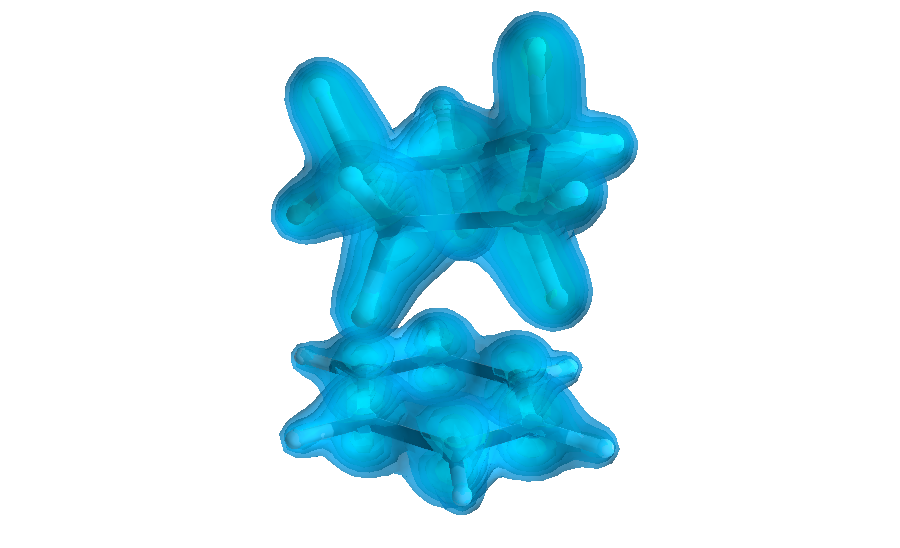
\includegraphics{Examples/benzcyclo_excite/sapt_dispersion_AB_e.png}
\caption{sapt\_dispersion\_AB\_g}
\end{figure}

    \hypertarget{ruxf3ux17cnica-dyspersji-miux119dzy-stanem-wzbudzonym-a-podstawowym}{%
\subsection{Różnica dyspersji między stanem wzbudzonym a
podstawowym}\label{ruxf3ux17cnica-dyspersji-miux119dzy-stanem-wzbudzonym-a-podstawowym}}

    Tak jak pokazano na poprzednich przykładach, ciężko jest czasem dostrzec
różnicę w dyspersji pomiędzy stanem podstawowym a stanem wzbudzonym.
Dlatego też program GVT potrafi policzyć różnicę gęstości czy też
dyspersji pomiędzy stanem podstawowym, a wzbudzonym, tak, że od wartości
dla stanu wzbudzonego odejmuje się wartości dla stanu podstawowego. Aby
to zrobić należy wczytać do programu GVT dane dla stanu podstawowego
oraz wzbudzonego tak jak w poprzednich przypadkach, a następnie wykonać:

    \begin{tcolorbox}[breakable, size=fbox, boxrule=1pt, pad at break*=1mm,colback=cellbackground, colframe=cellborder]
\prompt{In}{incolor}{27}{\boxspacing}
\begin{Verbatim}[commandchars=\\\{\}]
\PY{n}{sapt\PYZus{}dispersion\PYZus{}AB\PYZus{}eg} \PY{o}{=} \PY{o}{\PYZhy{}}\PY{p}{(} \PY{n}{sapt\PYZus{}dispersion\PYZus{}AB\PYZus{}e} \PY{o}{\PYZhy{}} \PY{n}{sapt\PYZus{}dispersion\PYZus{}AB\PYZus{}g} \PY{p}{)}
\PY{n}{X}\PY{p}{,} \PY{n}{Y}\PY{p}{,} \PY{n}{Z} \PY{o}{=} \PY{n}{sapt\PYZus{}A\PYZus{}e}\PY{o}{.}\PY{n}{orbital\PYZus{}generator}\PY{o}{.}\PY{n}{grid}\PY{o}{.}\PY{n}{return\PYZus{}grid\PYZus{}arrays}\PY{p}{(}\PY{p}{)}
\end{Verbatim}
\end{tcolorbox}

    \begin{tcolorbox}[breakable, size=fbox, boxrule=1pt, pad at break*=1mm,colback=cellbackground, colframe=cellborder]
\prompt{In}{incolor}{28}{\boxspacing}
\begin{Verbatim}[commandchars=\\\{\}]
\PY{n}{figure} \PY{o}{=} \PY{n}{visualization}\PY{o}{.}\PY{n}{mlab}\PY{o}{.}\PY{n}{figure}\PY{p}{(}  \PY{l+s+s2}{\PYZdq{}}\PY{l+s+s2}{sapt\PYZus{}dispersion\PYZus{}AB\PYZus{}eg}\PY{l+s+s2}{\PYZdq{}}\PY{p}{,} 
        \PY{n}{bgcolor}\PY{o}{=} \PY{n}{visualization}\PY{o}{.}\PY{n}{visualization\PYZus{}data}\PY{o}{.}\PY{n}{background\PYZus{}colors}\PY{p}{[}\PY{l+s+s1}{\PYZsq{}}\PY{l+s+s1}{White}\PY{l+s+s1}{\PYZsq{}}\PY{p}{]}\PY{p}{,}
        \PY{n}{size}\PY{o}{=}\PY{p}{(}\PY{l+m+mi}{900}\PY{p}{,} \PY{l+m+mi}{600}\PY{p}{)} \PY{p}{)}

\PY{n}{plot\PYZus{}figure} \PY{o}{=} \PY{n}{sapt\PYZus{}A\PYZus{}e}\PY{o}{.}\PY{n}{plot\PYZus{}orbitals\PYZus{}MO}\PY{p}{(}\PY{n}{orbital\PYZus{}numbers}\PY{o}{=}\PY{p}{[}\PY{p}{]}\PY{p}{,}\PY{n}{auto\PYZus{}show}\PY{o}{=}\PY{k+kc}{False}\PY{p}{,} 
    \PY{n}{plot\PYZus{}bonds}\PY{o}{=}\PY{k+kc}{True}\PY{p}{,} \PY{n}{atom\PYZus{}names}\PY{o}{=}\PY{k+kc}{False}\PY{p}{,} \PY{n}{atom\PYZus{}scaling}\PY{o}{=}\PY{l+m+mf}{0.5}\PY{p}{,} \PY{n}{figure} \PY{o}{=} \PY{n}{figure}\PY{p}{)}
\PY{n}{sapt\PYZus{}A\PYZus{}e}\PY{o}{.}\PY{n}{mlab}\PY{o}{.}\PY{n}{contour3d}\PY{p}{(} \PY{n}{X}\PY{p}{,} \PY{n}{Y}\PY{p}{,} \PY{n}{Z}\PY{p}{,} \PY{n}{sapt\PYZus{}dispersion\PYZus{}AB\PYZus{}eg}\PY{p}{,}  
\PY{n}{contours}\PY{o}{=} \PY{n}{sapt\PYZus{}A\PYZus{}e}\PY{o}{.}\PY{n}{contour\PYZus{}process}\PY{p}{(}\PY{p}{[}\PY{l+s+s1}{\PYZsq{}}\PY{l+s+s1}{70}\PY{l+s+s1}{\PYZpc{}}\PY{l+s+s1}{\PYZsq{}}\PY{p}{,}\PY{l+s+s1}{\PYZsq{}}\PY{l+s+s1}{50}\PY{l+s+s1}{\PYZpc{}}\PY{l+s+s1}{\PYZsq{}}\PY{p}{,}\PY{l+s+s1}{\PYZsq{}}\PY{l+s+s1}{40}\PY{l+s+s1}{\PYZpc{}}\PY{l+s+s1}{\PYZsq{}}\PY{p}{,}\PY{l+s+s1}{\PYZsq{}}\PY{l+s+s1}{30}\PY{l+s+s1}{\PYZpc{}}\PY{l+s+s1}{\PYZsq{}}\PY{p}{,}\PY{l+s+s1}{\PYZsq{}}\PY{l+s+s1}{20}\PY{l+s+s1}{\PYZpc{}}\PY{l+s+s1}{\PYZsq{}}\PY{p}{,}\PY{l+s+s1}{\PYZsq{}}\PY{l+s+s1}{10}\PY{l+s+s1}{\PYZpc{}}\PY{l+s+s1}{\PYZsq{}}\PY{p}{,}\PY{l+s+s1}{\PYZsq{}}\PY{l+s+s1}{1}\PY{l+s+s1}{\PYZpc{}}\PY{l+s+s1}{\PYZsq{}}\PY{p}{]}\PY{p}{,}
\PY{n}{sapt\PYZus{}dispersion\PYZus{}AB\PYZus{}eg}\PY{p}{)} \PY{p}{,} \PY{n}{opacity}\PY{o}{=}\PY{l+m+mf}{0.5}\PY{p}{)}
\PY{n}{sapt\PYZus{}A\PYZus{}e}\PY{o}{.}\PY{n}{mlab}\PY{o}{.}\PY{n}{view}\PY{p}{(} \PY{n}{distance}\PY{o}{=}\PY{l+m+mi}{26} \PY{p}{)}
\PY{c+c1}{\PYZsh{} sapt\PYZus{}A\PYZus{}e.mlab.savefig(filename= \PYZsq{}sapt\PYZus{}dispersion\PYZus{}AB\PYZus{}eg.png\PYZsq{})}

\PY{n}{sapt\PYZus{}A\PYZus{}e}\PY{o}{.}\PY{n}{mlab}\PY{o}{.}\PY{n}{show}\PY{p}{(}\PY{p}{)}
\end{Verbatim}
\end{tcolorbox}

    Przykład wizualizacji różnicy dyspersji dla stanów wzbudzonego i
podstawowego układu benzen-cyklopentan pokazano poniżej:

\begin{figure}
\centering
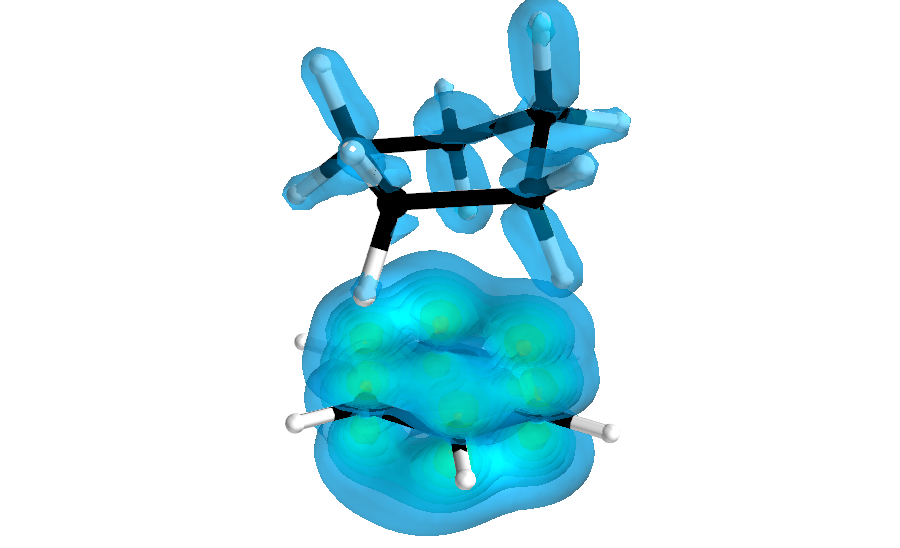
\includegraphics{Examples/benzcyclo_excite/sapt_dispersion_AB_eg.png}
\caption{sapt\_dispersion\_AB\_g}
\end{figure}

    \hypertarget{wizualizacji-ruxf3ux17cnicy-gux119stoux15bci-z-gvt-dla-wynikuxf3w-saptcas-obliczonych-za-pomocux105-molpro-oraz-gammcor}{%
\subsection{Wizualizacji różnicy gęstości z GVT dla wyników SAPT(CAS)
obliczonych za pomocą MOLPRO oraz
GAMMCOR}\label{wizualizacji-ruxf3ux17cnicy-gux119stoux15bci-z-gvt-dla-wynikuxf3w-saptcas-obliczonych-za-pomocux105-molpro-oraz-gammcor}}

    \begin{tcolorbox}[breakable, size=fbox, boxrule=1pt, pad at break*=1mm,colback=cellbackground, colframe=cellborder]
\prompt{In}{incolor}{29}{\boxspacing}
\begin{Verbatim}[commandchars=\\\{\}]
\PY{n}{sapt\PYZus{}density\PYZus{}A\PYZus{}g} \PY{o}{=}  \PY{n}{np}\PY{o}{.}\PY{n}{zeros\PYZus{}like}\PY{p}{(} \PY{n}{sapt\PYZus{}A\PYZus{}g}\PY{o}{.}\PY{n}{molecular\PYZus{}system}\PY{o}{.}\PY{n}{AOs}\PY{p}{[}\PY{l+m+mi}{0}\PY{p}{]} \PY{p}{)}
\PY{n}{sapt\PYZus{}density\PYZus{}B\PYZus{}g} \PY{o}{=}  \PY{n}{np}\PY{o}{.}\PY{n}{zeros\PYZus{}like}\PY{p}{(} \PY{n}{sapt\PYZus{}B\PYZus{}g}\PY{o}{.}\PY{n}{molecular\PYZus{}system}\PY{o}{.}\PY{n}{AOs}\PY{p}{[}\PY{l+m+mi}{0}\PY{p}{]} \PY{p}{)}
\PY{k}{for} \PY{n}{i} \PY{o+ow}{in} \PY{n+nb}{range}\PY{p}{(}\PY{n}{NOccupA\PYZus{}g}\PY{p}{)}\PY{p}{:}
    \PY{n}{sapt\PYZus{}density\PYZus{}A\PYZus{}g} \PY{o}{+}\PY{o}{=} \PY{n}{A\PYZus{}Occ\PYZus{}g}\PY{p}{[}\PY{n}{i}\PY{p}{]} \PY{o}{*} \PY{n}{sapt\PYZus{}A\PYZus{}g}\PY{o}{.}\PY{n}{molecular\PYZus{}system}\PY{o}{.}\PY{n}{MOs}\PY{p}{[}\PY{n}{i}\PY{p}{]}\PY{o}{*}\PY{o}{*}\PY{l+m+mi}{2} 
\PY{k}{for} \PY{n}{j} \PY{o+ow}{in} \PY{n+nb}{range}\PY{p}{(}\PY{n}{NOccupB\PYZus{}e}\PY{p}{)}\PY{p}{:}   
    \PY{n}{sapt\PYZus{}density\PYZus{}B\PYZus{}g} \PY{o}{+}\PY{o}{=} \PY{n}{B\PYZus{}Occ\PYZus{}g}\PY{p}{[}\PY{n}{j}\PY{p}{]} \PY{o}{*} \PY{n}{sapt\PYZus{}B\PYZus{}g}\PY{o}{.}\PY{n}{molecular\PYZus{}system}\PY{o}{.}\PY{n}{MOs}\PY{p}{[}\PY{n}{j}\PY{p}{]}\PY{o}{*}\PY{o}{*}\PY{l+m+mi}{2} 

\PY{n}{sapt\PYZus{}density\PYZus{}A\PYZus{}e} \PY{o}{=}  \PY{n}{np}\PY{o}{.}\PY{n}{zeros\PYZus{}like}\PY{p}{(} \PY{n}{sapt\PYZus{}A\PYZus{}e}\PY{o}{.}\PY{n}{molecular\PYZus{}system}\PY{o}{.}\PY{n}{AOs}\PY{p}{[}\PY{l+m+mi}{0}\PY{p}{]} \PY{p}{)}
\PY{n}{sapt\PYZus{}density\PYZus{}B\PYZus{}e} \PY{o}{=}  \PY{n}{np}\PY{o}{.}\PY{n}{zeros\PYZus{}like}\PY{p}{(} \PY{n}{sapt\PYZus{}B\PYZus{}e}\PY{o}{.}\PY{n}{molecular\PYZus{}system}\PY{o}{.}\PY{n}{AOs}\PY{p}{[}\PY{l+m+mi}{0}\PY{p}{]} \PY{p}{)}
\PY{k}{for} \PY{n}{i} \PY{o+ow}{in} \PY{n+nb}{range}\PY{p}{(}\PY{n}{NOccupA\PYZus{}e}\PY{p}{)}\PY{p}{:}
    \PY{n}{sapt\PYZus{}density\PYZus{}A\PYZus{}e} \PY{o}{+}\PY{o}{=} \PY{n}{A\PYZus{}Occ\PYZus{}e}\PY{p}{[}\PY{n}{i}\PY{p}{]} \PY{o}{*} \PY{n}{sapt\PYZus{}A\PYZus{}e}\PY{o}{.}\PY{n}{molecular\PYZus{}system}\PY{o}{.}\PY{n}{MOs}\PY{p}{[}\PY{n}{i}\PY{p}{]}\PY{o}{*}\PY{o}{*}\PY{l+m+mi}{2} 
\PY{k}{for} \PY{n}{j} \PY{o+ow}{in} \PY{n+nb}{range}\PY{p}{(}\PY{n}{NOccupB\PYZus{}e}\PY{p}{)}\PY{p}{:}      
    \PY{n}{sapt\PYZus{}density\PYZus{}B\PYZus{}e} \PY{o}{+}\PY{o}{=}  \PY{n}{B\PYZus{}Occ\PYZus{}e}\PY{p}{[}\PY{n}{j}\PY{p}{]} \PY{o}{*} \PY{n}{sapt\PYZus{}B\PYZus{}e}\PY{o}{.}\PY{n}{molecular\PYZus{}system}\PY{o}{.}\PY{n}{MOs}\PY{p}{[}\PY{n}{j}\PY{p}{]}\PY{o}{*}\PY{o}{*}\PY{l+m+mi}{2} 
\PY{n}{sapt\PYZus{}density\PYZus{}AB\PYZus{}g} \PY{o}{=} \PY{p}{(} \PY{n}{sapt\PYZus{}density\PYZus{}A\PYZus{}g} \PY{o}{+} \PY{n}{sapt\PYZus{}density\PYZus{}B\PYZus{}g} \PY{p}{)}  
\PY{n}{sapt\PYZus{}density\PYZus{}AB\PYZus{}e} \PY{o}{=} \PY{p}{(} \PY{n}{sapt\PYZus{}density\PYZus{}A\PYZus{}e} \PY{o}{+} \PY{n}{sapt\PYZus{}density\PYZus{}B\PYZus{}e} \PY{p}{)}  
\end{Verbatim}
\end{tcolorbox}

    Program GVT oblicza różnicę gęstości tak, że od stanu wzbudzonego
odejmuje wartości dla stanu podstawowego.

    \begin{tcolorbox}[breakable, size=fbox, boxrule=1pt, pad at break*=1mm,colback=cellbackground, colframe=cellborder]
\prompt{In}{incolor}{30}{\boxspacing}
\begin{Verbatim}[commandchars=\\\{\}]
\PY{n}{sapt\PYZus{}density\PYZus{}AB\PYZus{}eg} \PY{o}{=} \PY{p}{(} \PY{n}{sapt\PYZus{}density\PYZus{}AB\PYZus{}e} \PY{o}{\PYZhy{}} \PY{n}{sapt\PYZus{}density\PYZus{}AB\PYZus{}g} \PY{p}{)}
\end{Verbatim}
\end{tcolorbox}

    W ostatnim kroku wyświetlamy naszą różnicę gęstości. Użytkownik znów ma
dużą dowolność przy ustawieniu parametrów wyświetlania, tak jak to było
w poprzednich przykładach.

    \begin{tcolorbox}[breakable, size=fbox, boxrule=1pt, pad at break*=1mm,colback=cellbackground, colframe=cellborder]
\prompt{In}{incolor}{31}{\boxspacing}
\begin{Verbatim}[commandchars=\\\{\}]
\PY{n}{figure} \PY{o}{=} \PY{n}{visualization}\PY{o}{.}\PY{n}{mlab}\PY{o}{.}\PY{n}{figure}\PY{p}{(}  \PY{l+s+s2}{\PYZdq{}}\PY{l+s+s2}{sapt\PYZus{}density\PYZus{}AB\PYZus{}eg}\PY{l+s+s2}{\PYZdq{}}\PY{p}{,} 
        \PY{n}{bgcolor}\PY{o}{=} \PY{n}{visualization}\PY{o}{.}\PY{n}{visualization\PYZus{}data}\PY{o}{.}\PY{n}{background\PYZus{}colors}\PY{p}{[}\PY{l+s+s1}{\PYZsq{}}\PY{l+s+s1}{White}\PY{l+s+s1}{\PYZsq{}}\PY{p}{]}\PY{p}{,}
        \PY{n}{size}\PY{o}{=}\PY{p}{(}\PY{l+m+mi}{900}\PY{p}{,} \PY{l+m+mi}{600}\PY{p}{)} \PY{p}{)}

\PY{n}{X}\PY{p}{,} \PY{n}{Y}\PY{p}{,} \PY{n}{Z} \PY{o}{=} \PY{n}{sapt\PYZus{}A\PYZus{}e}\PY{o}{.}\PY{n}{orbital\PYZus{}generator}\PY{o}{.}\PY{n}{grid}\PY{o}{.}\PY{n}{return\PYZus{}grid\PYZus{}arrays}\PY{p}{(}\PY{p}{)}
\PY{n}{plot\PYZus{}figure} \PY{o}{=} \PY{n}{sapt\PYZus{}A\PYZus{}e}\PY{o}{.}\PY{n}{plot\PYZus{}orbitals\PYZus{}MO}\PY{p}{(}\PY{n}{orbital\PYZus{}numbers}\PY{o}{=}\PY{p}{[}\PY{p}{]}\PY{p}{,}\PY{n}{auto\PYZus{}show}\PY{o}{=}\PY{k+kc}{False}\PY{p}{,} 
    \PY{n}{plot\PYZus{}bonds}\PY{o}{=}\PY{k+kc}{True}\PY{p}{,} \PY{n}{atom\PYZus{}names}\PY{o}{=}\PY{k+kc}{False}\PY{p}{,} \PY{n}{atom\PYZus{}scaling}\PY{o}{=}\PY{l+m+mf}{0.5} \PY{p}{,} \PY{n}{figure} \PY{o}{=} \PY{n}{figure}\PY{p}{)}
\PY{n}{sapt\PYZus{}A\PYZus{}e}\PY{o}{.}\PY{n}{mlab}\PY{o}{.}\PY{n}{contour3d}\PY{p}{(}    \PY{n}{X}\PY{p}{,} \PY{n}{Y}\PY{p}{,} \PY{n}{Z}\PY{p}{,} \PY{n}{sapt\PYZus{}density\PYZus{}AB\PYZus{}eg}\PY{p}{,} 
                    \PY{n}{contours}\PY{o}{=} \PY{n}{sapt\PYZus{}A\PYZus{}e}\PY{o}{.}\PY{n}{contour\PYZus{}process}\PY{p}{(} 
                    \PY{p}{[}\PY{l+s+s1}{\PYZsq{}}\PY{l+s+s1}{70}\PY{l+s+s1}{\PYZpc{}}\PY{l+s+s1}{\PYZsq{}}\PY{p}{,}\PY{l+s+s1}{\PYZsq{}}\PY{l+s+s1}{60}\PY{l+s+s1}{\PYZpc{}}\PY{l+s+s1}{\PYZsq{}}\PY{p}{,}\PY{l+s+s1}{\PYZsq{}}\PY{l+s+s1}{50}\PY{l+s+s1}{\PYZpc{}}\PY{l+s+s1}{\PYZsq{}}\PY{p}{,}\PY{l+s+s1}{\PYZsq{}}\PY{l+s+s1}{40}\PY{l+s+s1}{\PYZpc{}}\PY{l+s+s1}{\PYZsq{}}\PY{p}{,}\PY{l+s+s1}{\PYZsq{}}\PY{l+s+s1}{30}\PY{l+s+s1}{\PYZpc{}}\PY{l+s+s1}{\PYZsq{}}\PY{p}{,}\PY{l+s+s1}{\PYZsq{}}\PY{l+s+s1}{20}\PY{l+s+s1}{\PYZpc{}}\PY{l+s+s1}{\PYZsq{}}\PY{p}{,}\PY{l+s+s1}{\PYZsq{}}\PY{l+s+s1}{10}\PY{l+s+s1}{\PYZpc{}}\PY{l+s+s1}{\PYZsq{}}\PY{p}{,}\PY{l+s+s1}{\PYZsq{}}\PY{l+s+s1}{1}\PY{l+s+s1}{\PYZpc{}}\PY{l+s+s1}{\PYZsq{}}\PY{p}{,}\PY{l+s+s1}{\PYZsq{}}\PY{l+s+s1}{0.1}\PY{l+s+s1}{\PYZpc{}}\PY{l+s+s1}{\PYZsq{}}\PY{p}{]}\PY{p}{,} 
                    \PY{n}{sapt\PYZus{}density\PYZus{}AB\PYZus{}eg}\PY{p}{)}\PY{p}{,} \PY{n}{opacity}\PY{o}{=}\PY{l+m+mf}{0.5}\PY{p}{)}
\PY{n}{sapt\PYZus{}A\PYZus{}e}\PY{o}{.}\PY{n}{mlab}\PY{o}{.}\PY{n}{view}\PY{p}{(} \PY{n}{distance}\PY{o}{=}\PY{l+m+mi}{26} \PY{p}{)}
\PY{c+c1}{\PYZsh{} sapt\PYZus{}A\PYZus{}e.mlab.savefig(filename= \PYZsq{}sapt\PYZus{}density\PYZus{}AB\PYZus{}eg.png\PYZsq{})}

\PY{n}{sapt\PYZus{}A\PYZus{}e}\PY{o}{.}\PY{n}{mlab}\PY{o}{.}\PY{n}{show}\PY{p}{(}\PY{p}{)}
\end{Verbatim}
\end{tcolorbox}

    Przykład wizualizacji różnicy gęstości elektronowych dla stanów
wzbudzonego i podstawowego układu benzen-cyklopentan pokazano poniżej:

\begin{figure}
\centering
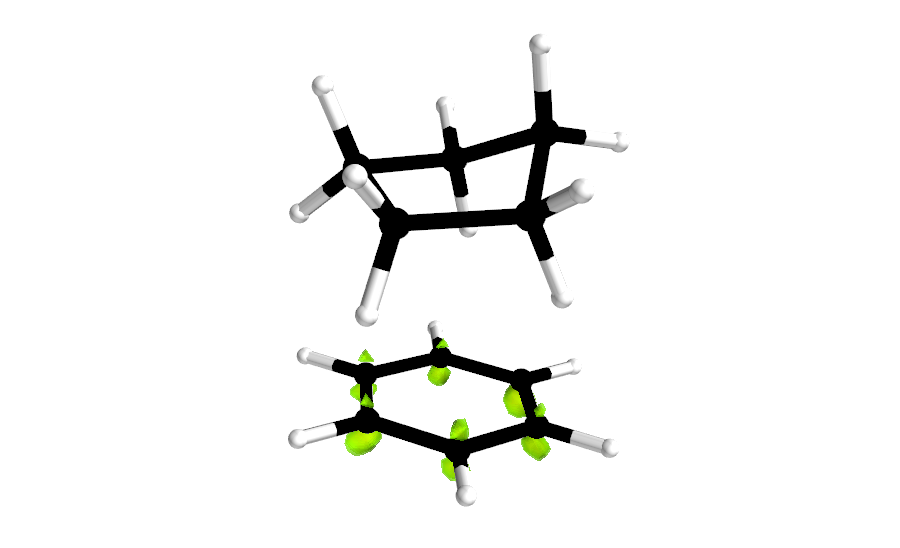
\includegraphics{Examples/benzcyclo_excite/sapt_density_AB_eg.png}
\caption{sapt\_dispersion\_AB\_g}
\end{figure}

    


    % Add a bibliography block to the postdoc
    
    
    
\end{document}
